\section{Gravitational waves}
``Space-time tells mass how to move; mass tells space-time how to curve" can provide a concise and sufficient summarization of Einstein's theory of general relativity (GR) ~\cite{Misner1973}. While providing the most complete theory of gravity to date, GR provides tools that allow considerations of high energy astrophyical phenomena (highly massive binary coalescences, spherically assymetric compact objects, etc.) whose fractional mass/energy output generates distortions in space-time known as gravitational waves. 
This is represented as a perturbation ($|h_{\mu \nu}|<<1$) in the Minkowski metric tensor defining a local linearized space-time:
\\
$$g_{\mu \nu} = \eta_{\mu \nu} + h_{\mu \nu}$$
\\
The wave-like behavior for $h_{\mu \nu}$ is realized after imposing the Lorentz gauge; producing 10 harmonic wave amplitudes from the Einstein field equations. Imposing a wave vector ($k_j$) onto one of three linearly independent spatial coordinates ($h^{ij}k_j$), the non-trivial amplitudes from the equations imply a transverse and traceless ($h^{i}_{i}$) gauge:
\\
$$\nabla^2 h_{+} - \frac{1}{c^2} \frac{\partial}{\partial t} h_{+} = 0$$
$$\nabla^2 h_{\times} - \frac{1}{c^2} \frac{\partial}{\partial t} h_{\times} = 0$$
\\
In other words, there exists a wave solution with two separate transverse polarizations $h_{+}$ and $h_{\times}$ with a $45^{\circ}$ separation between them. 

\textcolor{red}{Insert figure with the two gravitational wave polarizations and influence on spacetime}

When measured and analyzed, these waves can allow astronomers to extract novel information from the progenitors through the testing of various hypotheses pertinant to the violent dynamics of these systems. On September 14th, 2015 the Laser Interferometric Gravitational Wave Observatories detected the first direct gravitational wave from a pair of coalescing black holes 1.3 billion light years away, and since then other gravitational wave detectors (i.e. Virgo, KAGRA) have joined the search; continuing the search for novel events. This GW detector network has developed a track record with an ever increasing rate of detections including the first multimessenger event ~\cite{gw170817} and a suprising population of compact binary coalescences ~\cite{Nitz_2023}. The incredible perseverence of the women and men participating in this multi-decade effort dedicated to constructing and developing the large scale gravitational wave observatories used today is a testament to their resiliency and that of a curious mind. Though I fear I might insult or possibly bore an experienced reader with verbose and elementary material, personal curiosity has lead me to traverse the works of those before me and I do so with the most outspoken reverence; all while attempting my best to provide context of the novel contributions noted within this document. 

\newpage

\section{Detector configurations}
The current gravitational wave detector network primarily uses terrestrial bound Dual-Recycled Fabry-Perot Michelson interferometers; though to configure them into a state of observing, fundamental modes of operation are to be acquired first. We quickly review these modes to inform some of the basic ``whats'' and ``hows'' of detector operation with the hopes of developing a holistic view of the LIGO detection schema especially as it pertains to the body of this work. Most introductory detector configuration discussions start with the michelson interferometer and end at the dual-recycled Fabry-Perot Michelson interferometer; this section follows in kind. Alongside the discussion are citations which can provide exceptional alternative and more detailed explanations of topics discussed.

\subsection{Interferometry with a Michelson configuration}
``The Michelson'' interferometric detection schema, used by Michelson and Morley to test for the existence of luminiferous aether, demonstrates an inherent potential for measuring gravitational wave amplitudes generated by time varying quadrapole moments with high energy astrophysical progenitors; making it a prime candidate as a gravitational wave detector / observatory. The interferometry begins with a beam of coherent laser light split at a 50/50 beamsplitter along two perpendicular beam paths with respective lengths $L_x$ and $L_y$ that are set by highly reflective end mirrors. Upon arrival at the length terminating mirrors, the respective beams are back-reflected towards the beam splitter where they are made to interfere. The fringe power from this interference is measured at the anti-symmetric port 

%% Differential changes between the two optical path lengths can be tracked at the (anti-symmetric) by means of a differential change in the power ($P_\mathrm{out}$) measured at the detection port:

\begin{equation}\label{P_MICH_AS}
	P_\mathrm{out} = \frac{P_\mathrm{in}}{2} \bigg[1+\mathrm{cos}\Big(\frac{4\pi}{\lambda} (L_x - L_y)\Big) \bigg]
\end{equation}

The Michelson detects microsocopic differential length changes on the order of a fractional wavelength of the light used and are more aptly discussed as changes in differential phase ($\Delta \phi(t)$) between the returning perpendicular phasefronts ($\phi_x(t)$, $\phi_y(t)$). Understanding this inherent method of detection, a time-varying metric perturbation ($h(t)$), like that generated from a gravitational wave, is tested on a Michelson interferometer with a nominal arm length of L and a laser with optical angular frequency of $\Omega$:

\begin{equation}
\Delta \phi(t) = \phi_x(t) - \phi_y(t) =  \int_{t-2L/c}^{t} \Omega \bigg[1 + \frac{1}{2}h(t)\bigg]dt - \int_{t-2L/c}^{t} \Omega \bigg[1 - \frac{1}{2}h(t)\bigg]dt 
\end{equation}

Evaluating the above as a function of frequency yields:

\begin{equation}\label{MICH_del_phi}
	\Delta \phi (\omega) = h_0\frac{2 L \Omega}{c}e^{-i L \omega / c} \frac{\mathrm{sin}(L \omega /c)}{L \omega /c} = h_0 \cdot H(\omega, \phi_0)
\end{equation}

With the wave amplitude $h_0$, angular frequency $\omega$, nominal interferometer arm length $L$, speed of light $c$, and optical angular frequency $\Omega$.

The differential phase \ref{MICH_del_phi} combined with the power at the anti-symmetric port \ref{P_MICH_AS} provides a function of optical gain, dependent on freqency and a differential offset phase ($\phi_0$):

\begin{equation}
	\Delta P(\omega, \phi_0) = h_0 \frac{P_\mathrm{in}}{2} \Delta \phi (\omega) \cdot \mathrm{sin}(\phi_0)
\end{equation}

\begin{figure}[ht!]
	\begin{subcaptiongroup}
		\includegraphics[width=.45\textwidth,page=2]{INTRO/ifo_configs.pdf}
		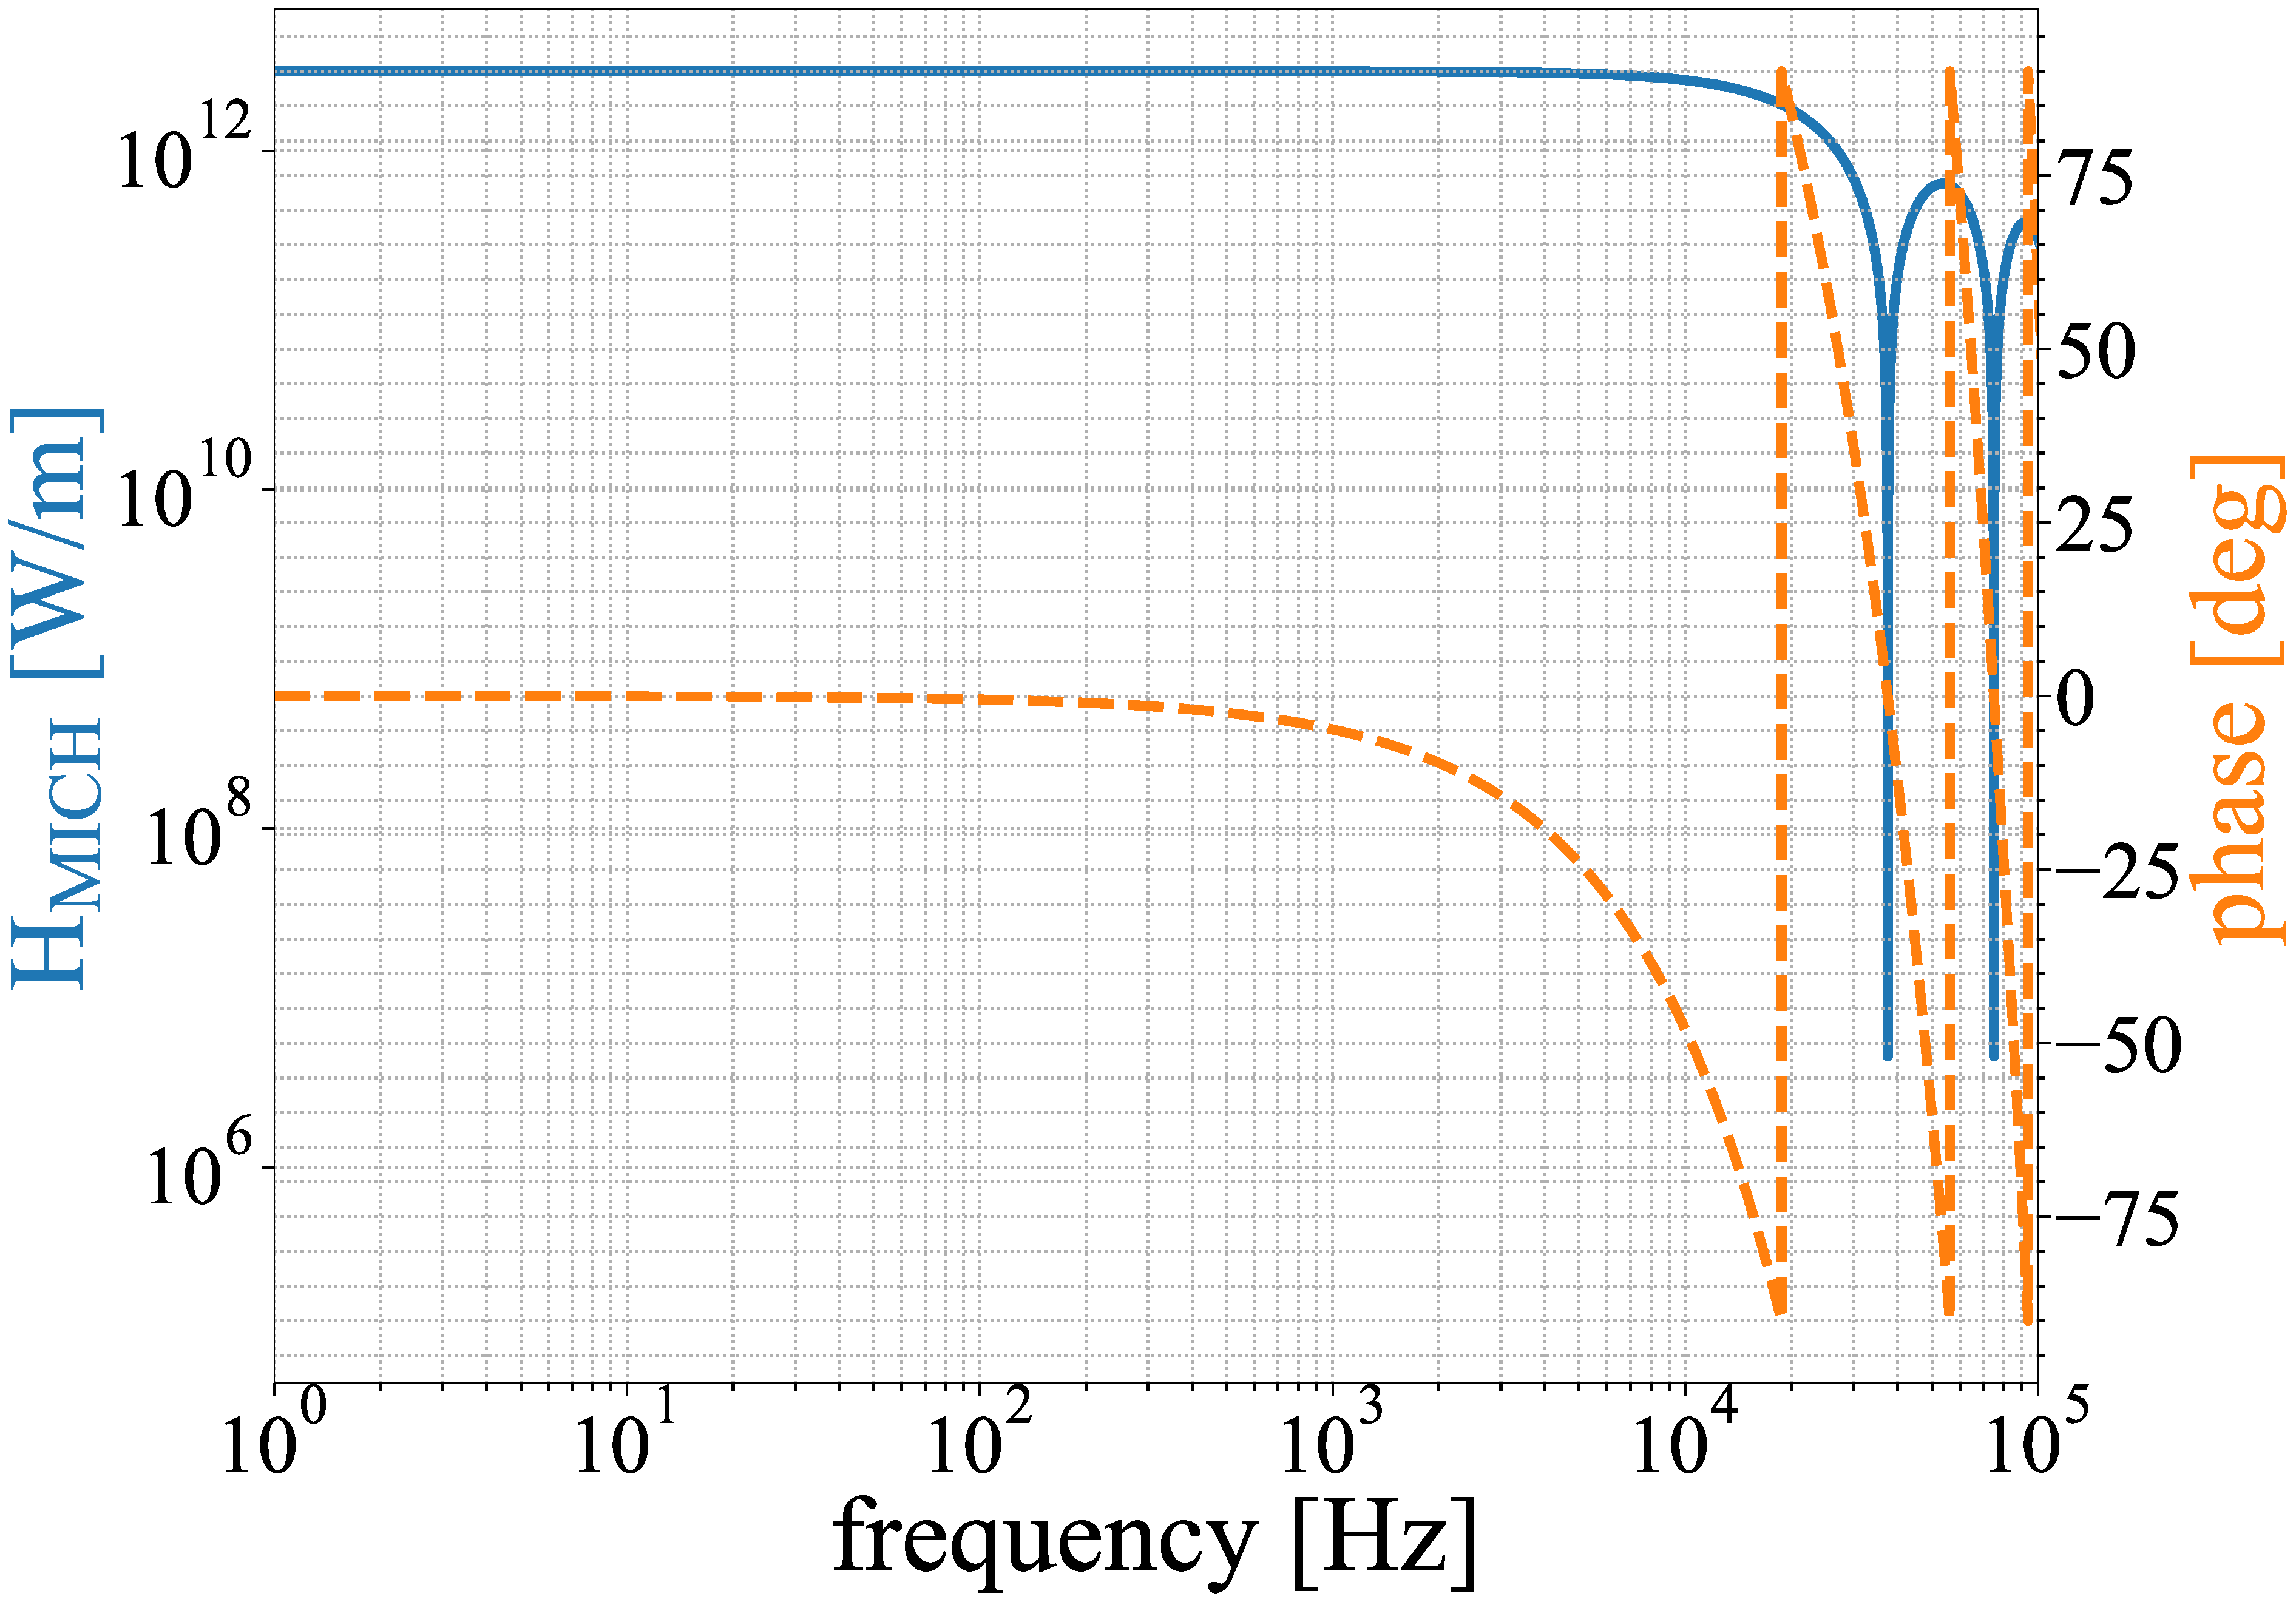
\includegraphics[width=.575\textwidth]{INTRO/mich_fr.pdf}
 	\end{subcaptiongroup}
  	\hfill
	\caption{[Left] A simplified schematic of a Michelson interferometer. [Right] The associated optical transfer function with $H(\omega, \pi/2)$ defining the optical gain of a Michelson interferometer with 4 km long arms and an input power of 25 [W]}
	\label{fig:mich}
\end{figure}
\FloatBarrier

Assuming a 4km arm configuration with 25 Watts input power as indicated in figure \ref{MICH_del_phi} the differential arm response provides a reasonable optical gain with the notches coorelating to an integer number of gravitational wave half periods ($\mathrm{n}\lambda_{gw} / 2$) to the interferometer arm length in such a way that the response is null. Though with sights set on optimizing detection bandwidth for neutron star binaries @ 100 Hz, the basic Michelson optical gain remains insufficient with enhancements required.  

\begin{figure}[ht!]
	\centering
	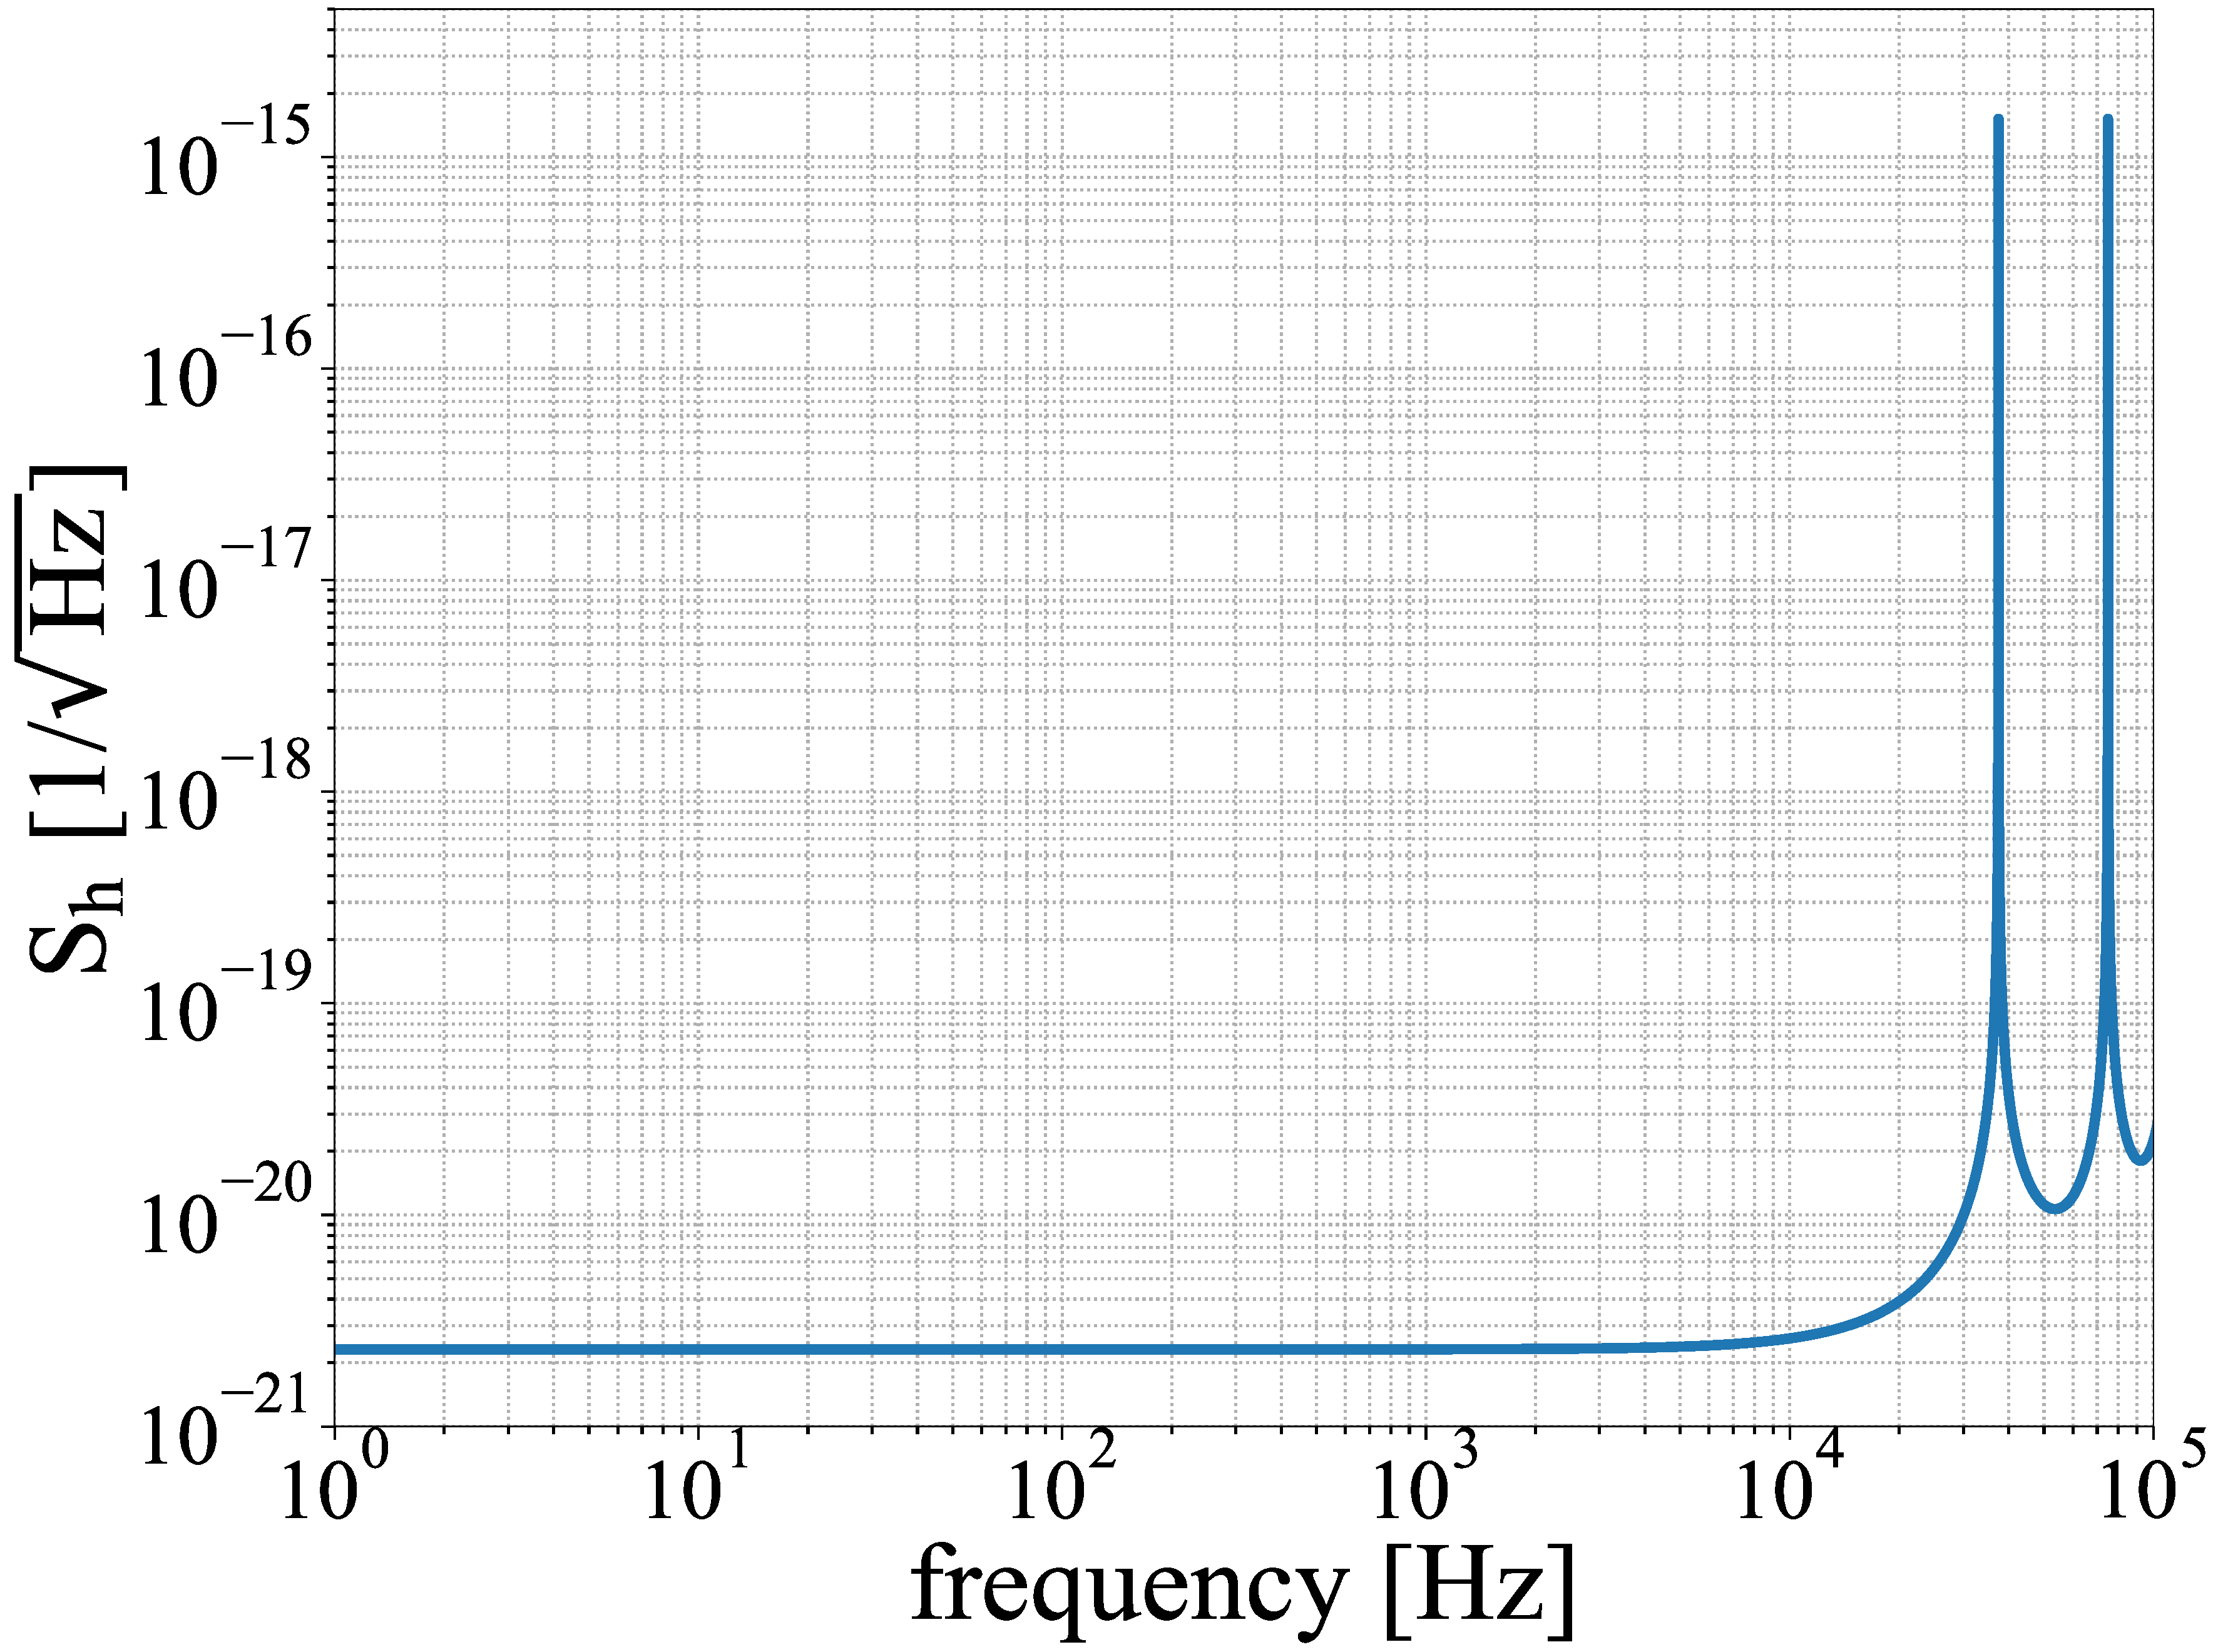
\includegraphics[width=\textwidth]{INTRO/mich_sensi.pdf}
	\caption{The shot noise~\ref{} limited sensitivity ($\sqrt{\hbar \Omega P_\mathdefault{in}}$ of a Michelson with 4 km long arms and an input power of 25 [W]. Compared to the apriori estimate of $10^{-21} \; [\frac{1}{\sqrt{\mathrm{Hz}}}]$ the signal to noise (SNR) comes to be unity. The desired confidence is set at a much higher standard with more unquestionable measurements set at SNR = 5.}
	\label{fig:michsensitivity}
\end{figure}

\subsubsection{Mode overlap}
Highly idealized depictions of interferometers can implicitly suggest their function and operation by planar phasefronts (for pedagogical purposes), though this assumption does not fully inform the reality. Defining the used laser carrier ''mode" with wavelength $\lambda$, and propogation axis ($z$); that being the Gaussian beam (TEM00 mode):

\begin{equation}\label{eq:gaussian_beam}
E(r) = E_o \frac{\sqrt{[\lambda z_o] / \pi}}{W(z)}e^{-r^2 / W^2(z)} e^{-ikz - ik[r^2 / (2R(z))] + i \zeta}
\end{equation}

Where $E_o$ is the complex field amplitude, $r^2/(2(R(z))$ defines the transverse coordinates $r^2$ on the hemisphere, with the ROC of $R(z)$, that defines a surface of uniform phase, $k$ is the wave number, $W(z)$ is the radius from the beam axis that contains (1-1/e^2)*100 \% of the integrated beam power, and $\zeta$ is the Gouy phase.

Shown in \ref{eq:gaussian_beam} is another propogation consideration that implies another symmetry required to be maintained of the co-propogating beams for optimal interference, and wavefront distortions / aberrations and their many forms are realized. Assymetric couplings are more often than not are introduced assymetrically between the orthogonal paths that often limit interference. Two metrics are used to describe how well this interference can is performed is set by ajnd contrast ($\nu$) and mode overlap ($\eta$): 

\begin{equation}\label{eq:mode_overlap}
	\eta = \bigg|\int E_x E_y dA \bigg|^{2} \bigg/ (P_x P_y)
\end{equation}

\begin{equation}\label{eq:contrast}
	\nu = \frac{P_\mathrm{max} - P_\mathrm{min}}{P_\mathrm{max} + P_\mathrm{min}}
\end{equation}

Contrast quantifies measured dark fringe power against the measured bright fringe power; while $\eta$ in the interferometric context produces a similar quantity by integration of phasefront overlap share matching phase the same phase phase front phasefront matching of the returning phasefronts at the beam splitter. Both these quantities operate on a scale of 0 to 1, from no to maximum interference though with one subtle difference. Mode overlap that being the morphology of resulting interference pattern for values less than 1. 

\textcolor{red}{FIGURE: Nonideal interference can result in generating any one of the provided interference patterns. Laguerre-Gauss and Hermite Gauss modes are metrics of mode mismatch and misalignment respectively.}

An important consideration for any sufficiently long arm length (like that used for LIGO), you are likely to encounter constraints in length if not without a sufficiently large beamsplitter and/or focusing optics. LIGO achieves this with curved end mirrors that match and focus the impinging wavefronts, though with a sensitivity indicated by ~\cite{} [$\mathrm{sensitivity} ~ 1/G_\mathrm{MICH} \approx 10^{-18} \; [\frac{1}{\sqrt{\mathrm{Hz}}}]]$ it still does not reach the requirement to confirm a measurement from CBCs @ 100 Hz ($\approx 10^{-21} \; [\frac{1}{\sqrt{\mathrm{Hz}}}]$.)

\subsection{Fabry-P\'{e}rot Michelson (FPMI)}
At the time of the LIGO proposal, constraints (physical and financial) for terrestrial gravitational wave detectors required a compact solution for increasing length (L) of the Michelson arms so to increase the beam phasefront lifetime within the Michelson arms. Two proposed arm folding techniques were considered: the Herriot Delay Line and the Fabry-P\'{e}rot cavity, though ultimately the Fabry-P\'{e}rot cavity is currently the predominent choice.

\begin{figure}[ht!]
	\centering
	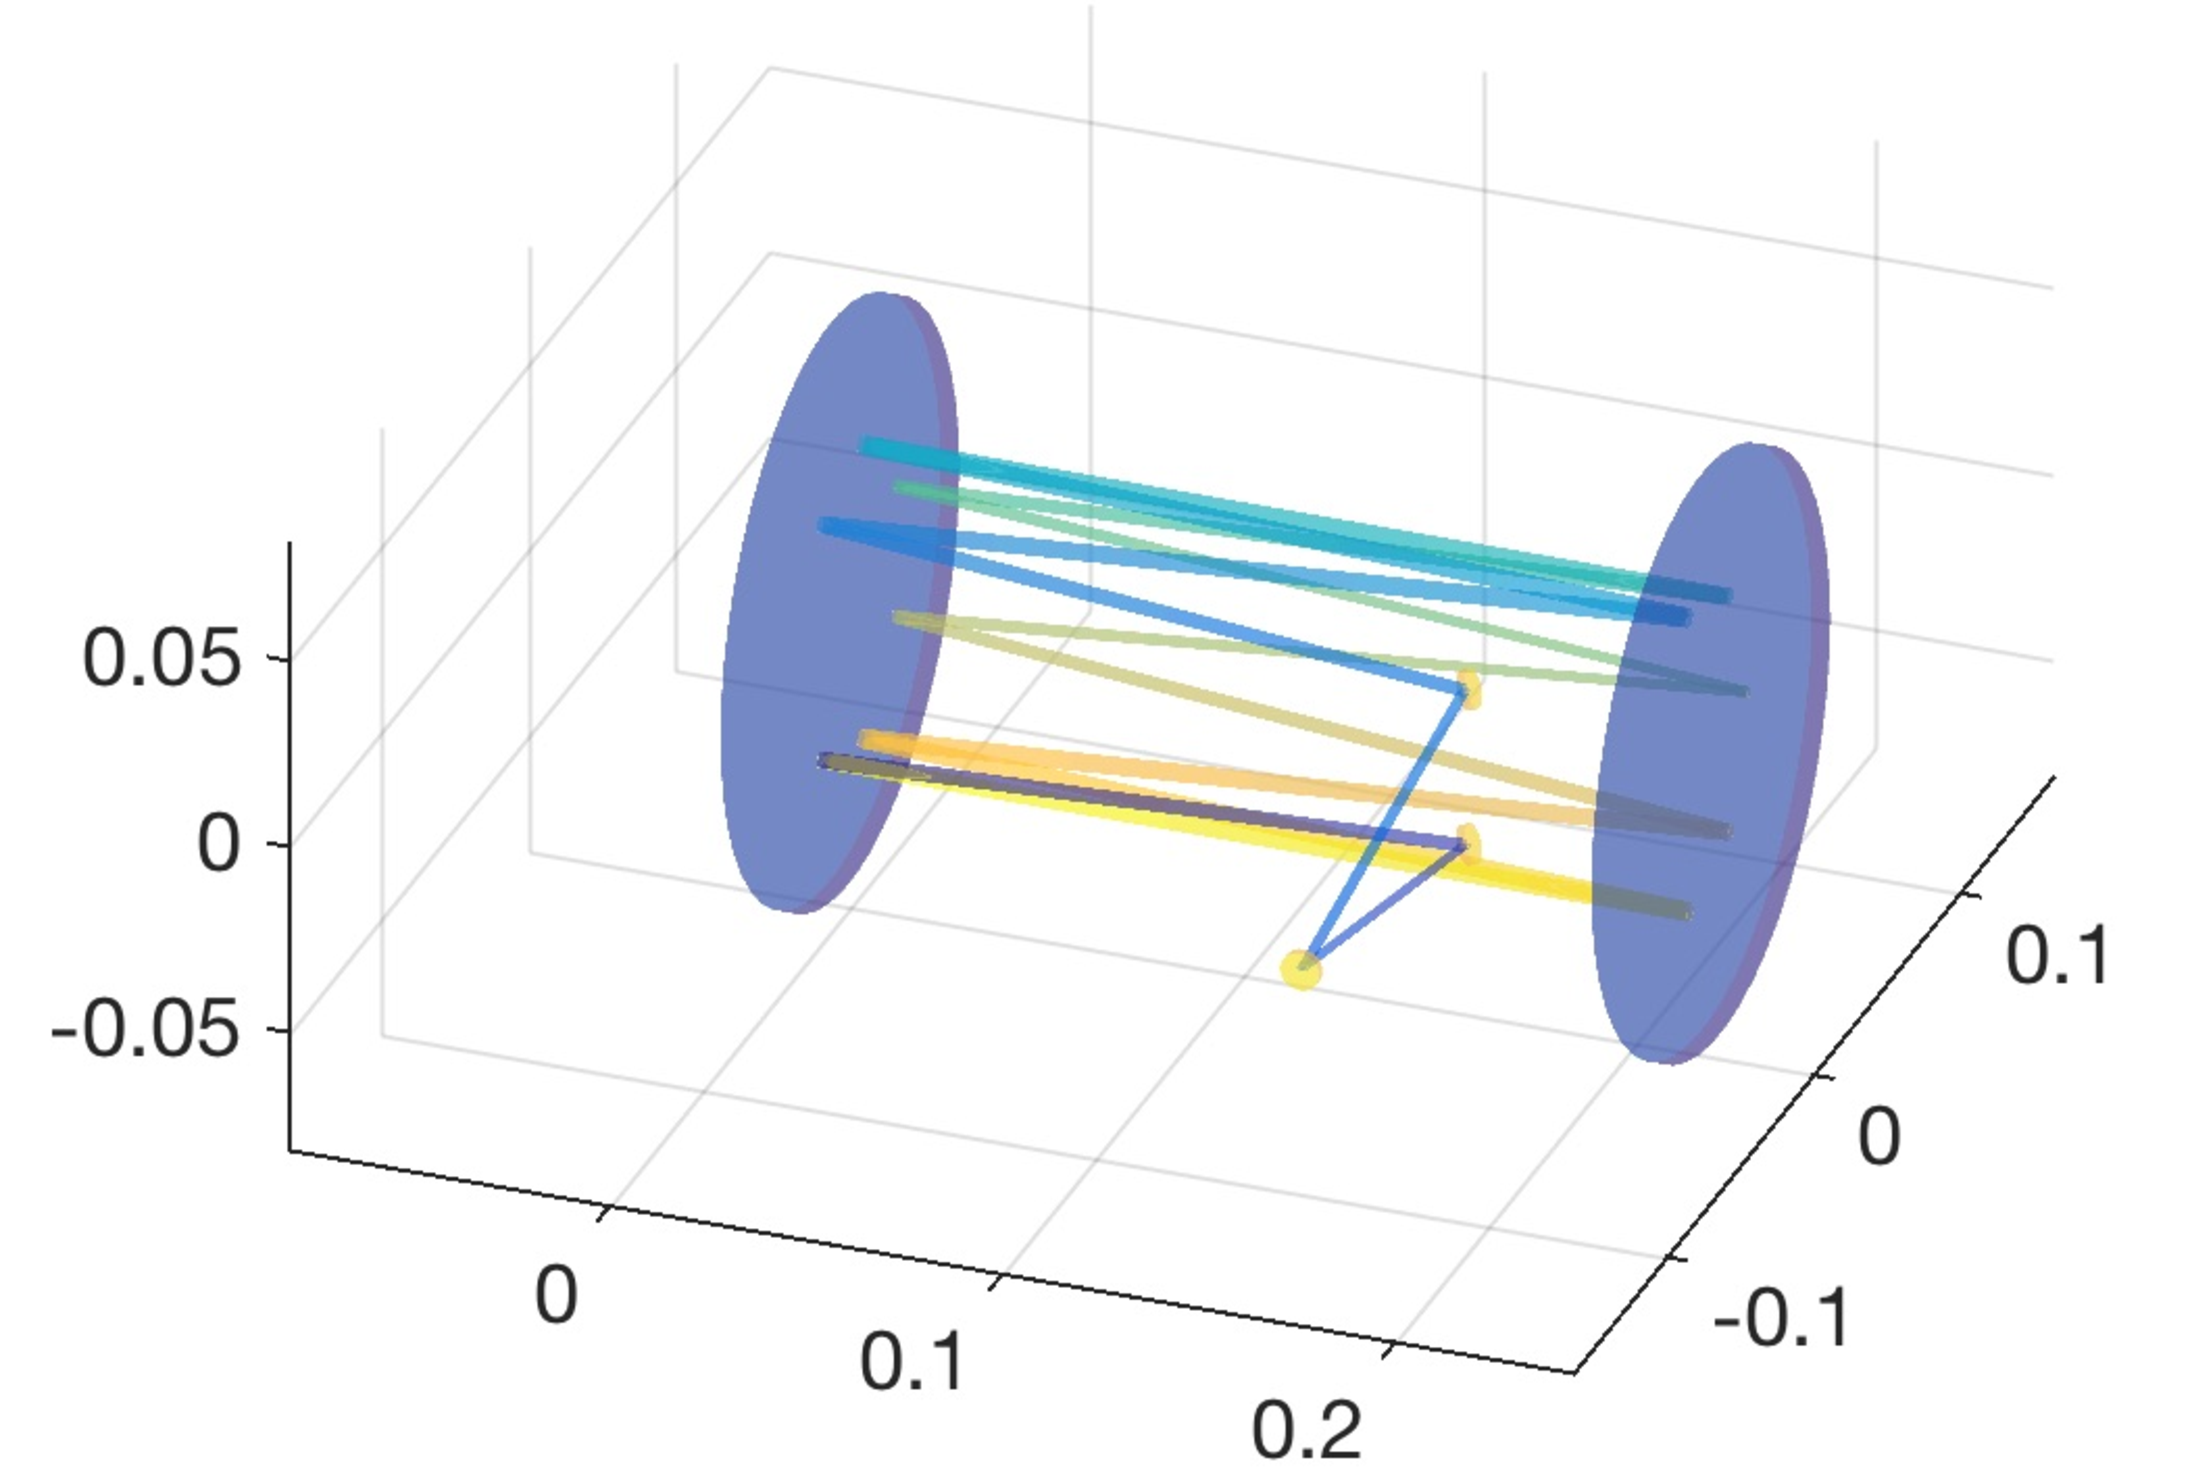
\includegraphics[width=\textwidth]{INTRO/HDL.pdf}
	\caption{A 12 bounce Herriot Delay Line with a small mirror input / output couplers inserted into the beam path.}
	\label{fig:hdl_cav}
\end{figure}


\subsubsection{The Fabry-P\'{e}rot cavity}
\label{section:FPC}
To understand the relevance of the Fabry-P\'{e}rot, we consider an idealized coherent light wave encountering an optical cavity with input and output mirror transmission and reflection coefficients of $t_1$, $r_1$ and $t_2$, $r_2$ respectively (and lossless mirrors $l=0$).

\begin{figure}[ht!]
	\centering
	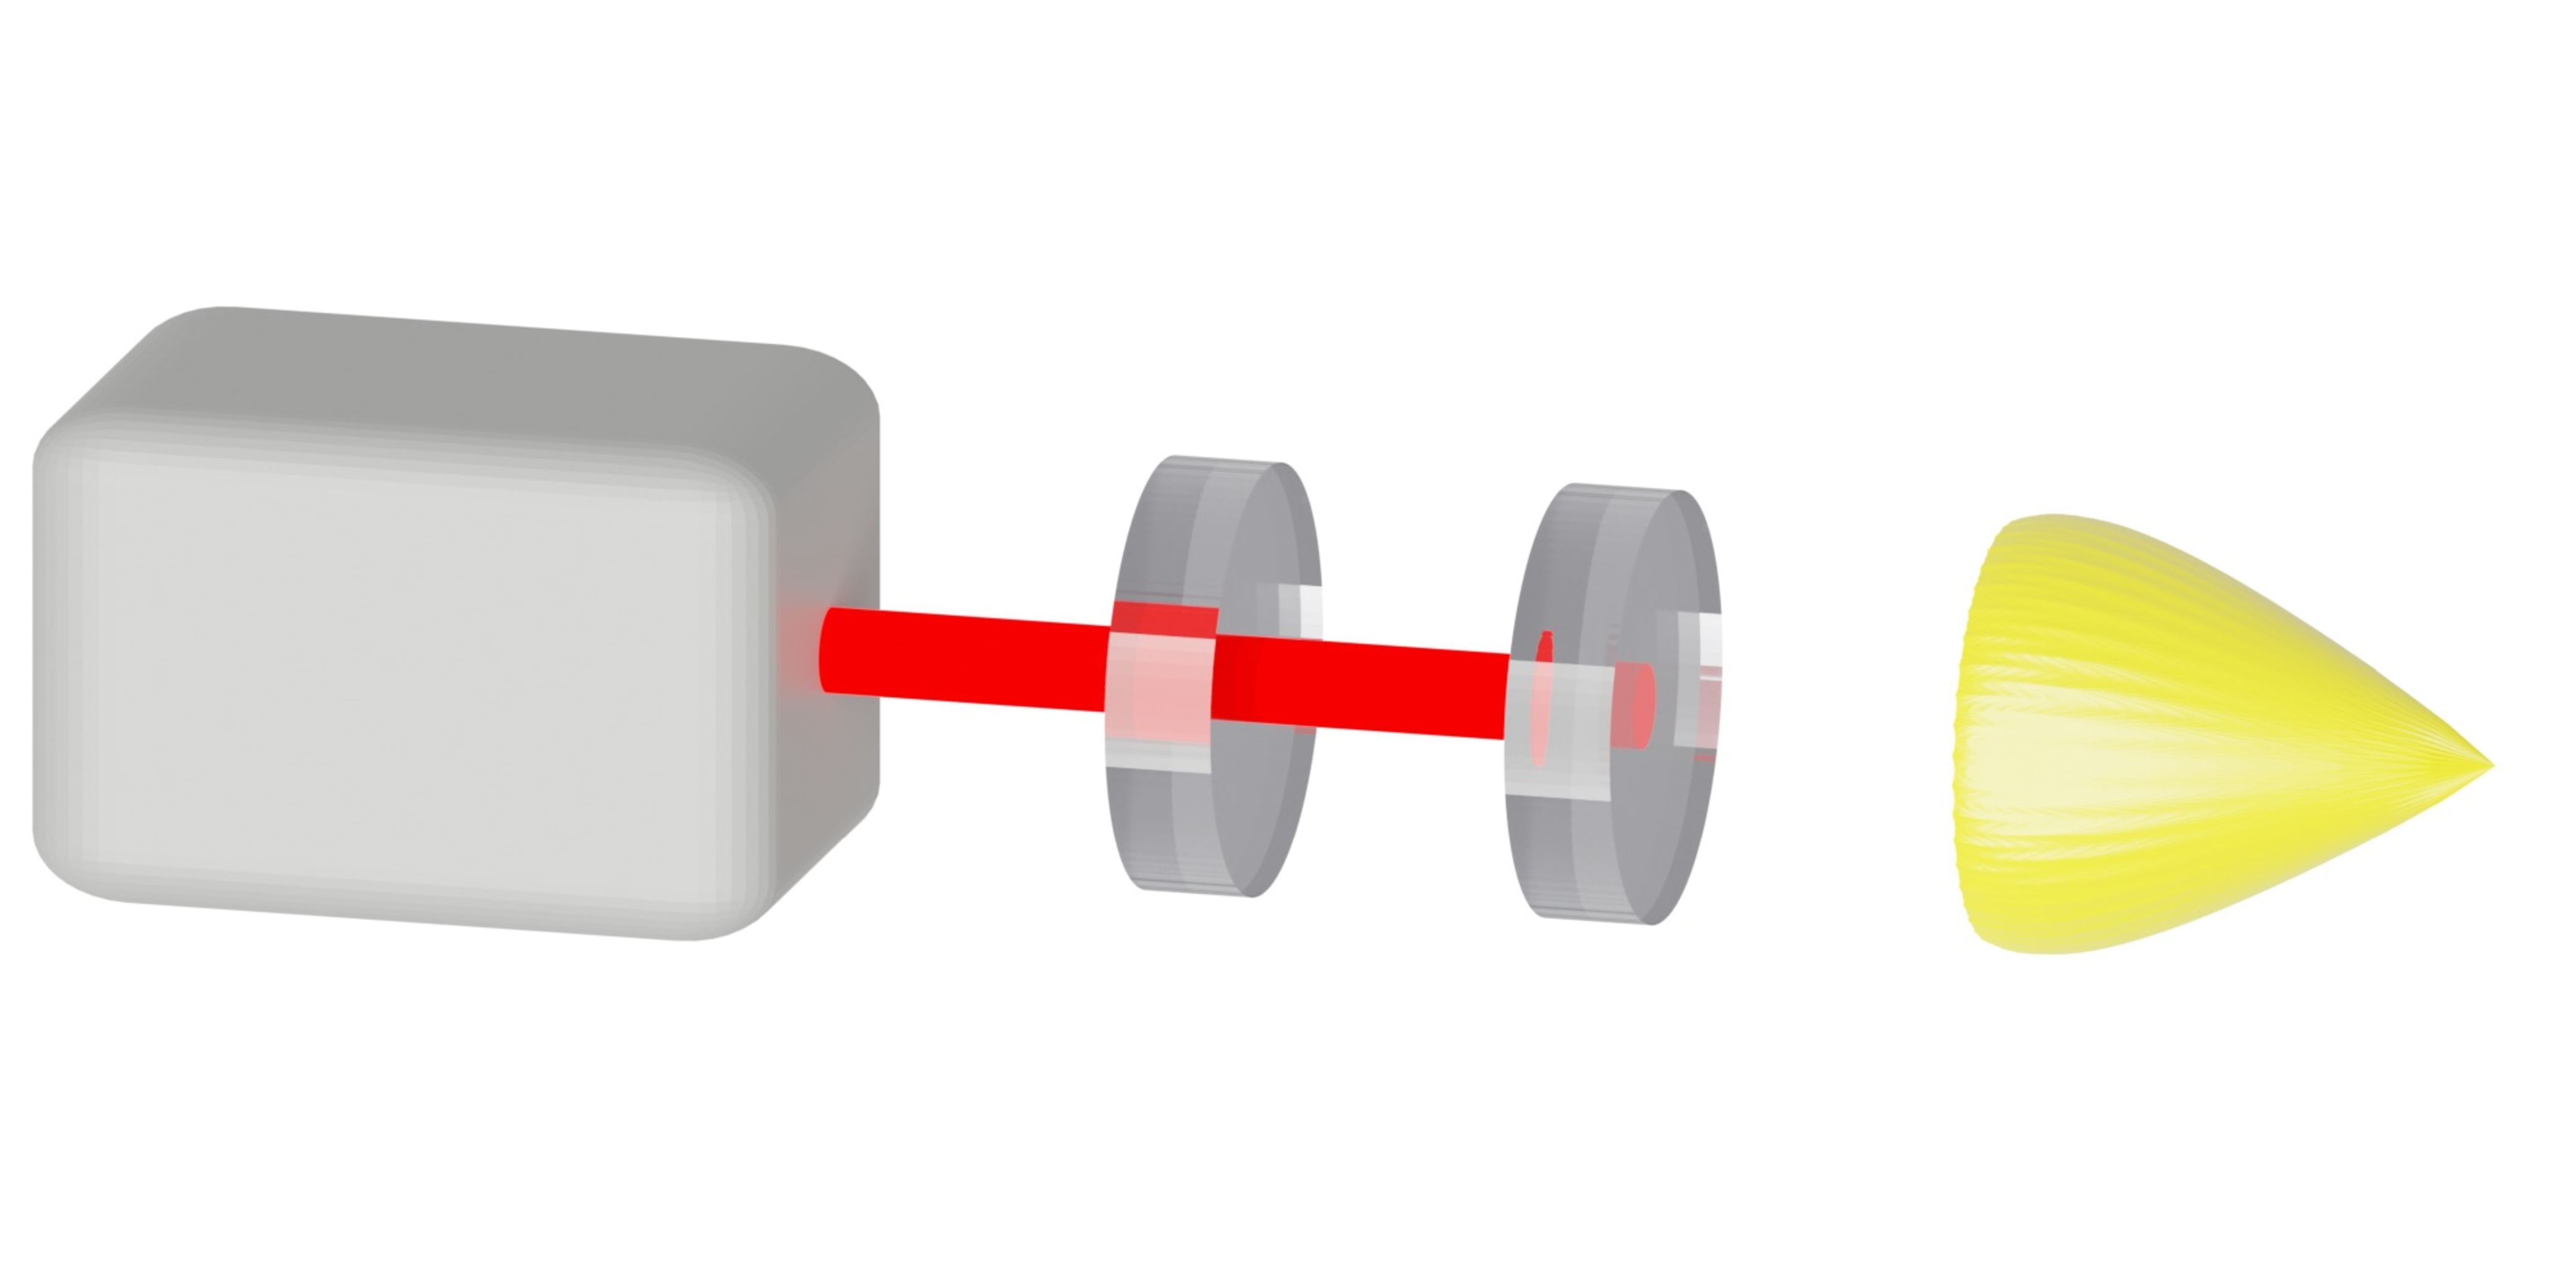
\includegraphics[width=\textwidth]{INTRO/simple_fp_alt_mid.pdf}
	\caption{Figure of a Fabry Perot Cavity. \textcolor{red}{Add HR surface to ITM and ETM. With a faint transmission beam to the more deliberately labeled transmission photodiode}}
	\label{fig:fp_cav}
\end{figure}

Light enters the cavity only after passing the input mirror with the incident field amplitude reduced by the mirror reflection coefficient. Though seemingly not useful, it is with an integer number of wavelengths of the incident laser light between the two mirrors that the circulating beam coherently adds with the input, achieving resonance.  A cavity of length $L$ and comprised of an input coupler ($r_1$,$t_1$) and end mirror ($r_2$, $t_2$) yield the following effective cavity reflection and transmission coefficients: 

\iffalse that the input and circulating that the photons belonging to a particular phasefront can be experimentally tracked, and lucky for us this is is why we measure interference at the anti-symmetric port. But these benefit with a constant source at the cavity input the phasefronts entering the cavity are superimposed onto the circulating cavity field and, more often than not, add incoherently which can makes this thought experiment seem silly.\fi 

\begin{equation}
	r_c = -r_1 + \frac{t^2_1r_2 e^{-i2kL}}{1-r_1 r_2 e^{-i2kl}}
\end{equation}

\begin{equation}
	t_c = \frac{t_1 t_2 e^{-ikL}}{1-r_1 r_2 e^{-i2kL}}	
\end{equation}

Tuning the positions of mirrors with high reflectivity coefficients and the usage of an infared laser (i.e. $\lambda$ 1064nm) requires strict length tuning and maintenance for resonance ($\leq 1\mathrm{e-}7$ [m]). 

\begin{figure}[H]
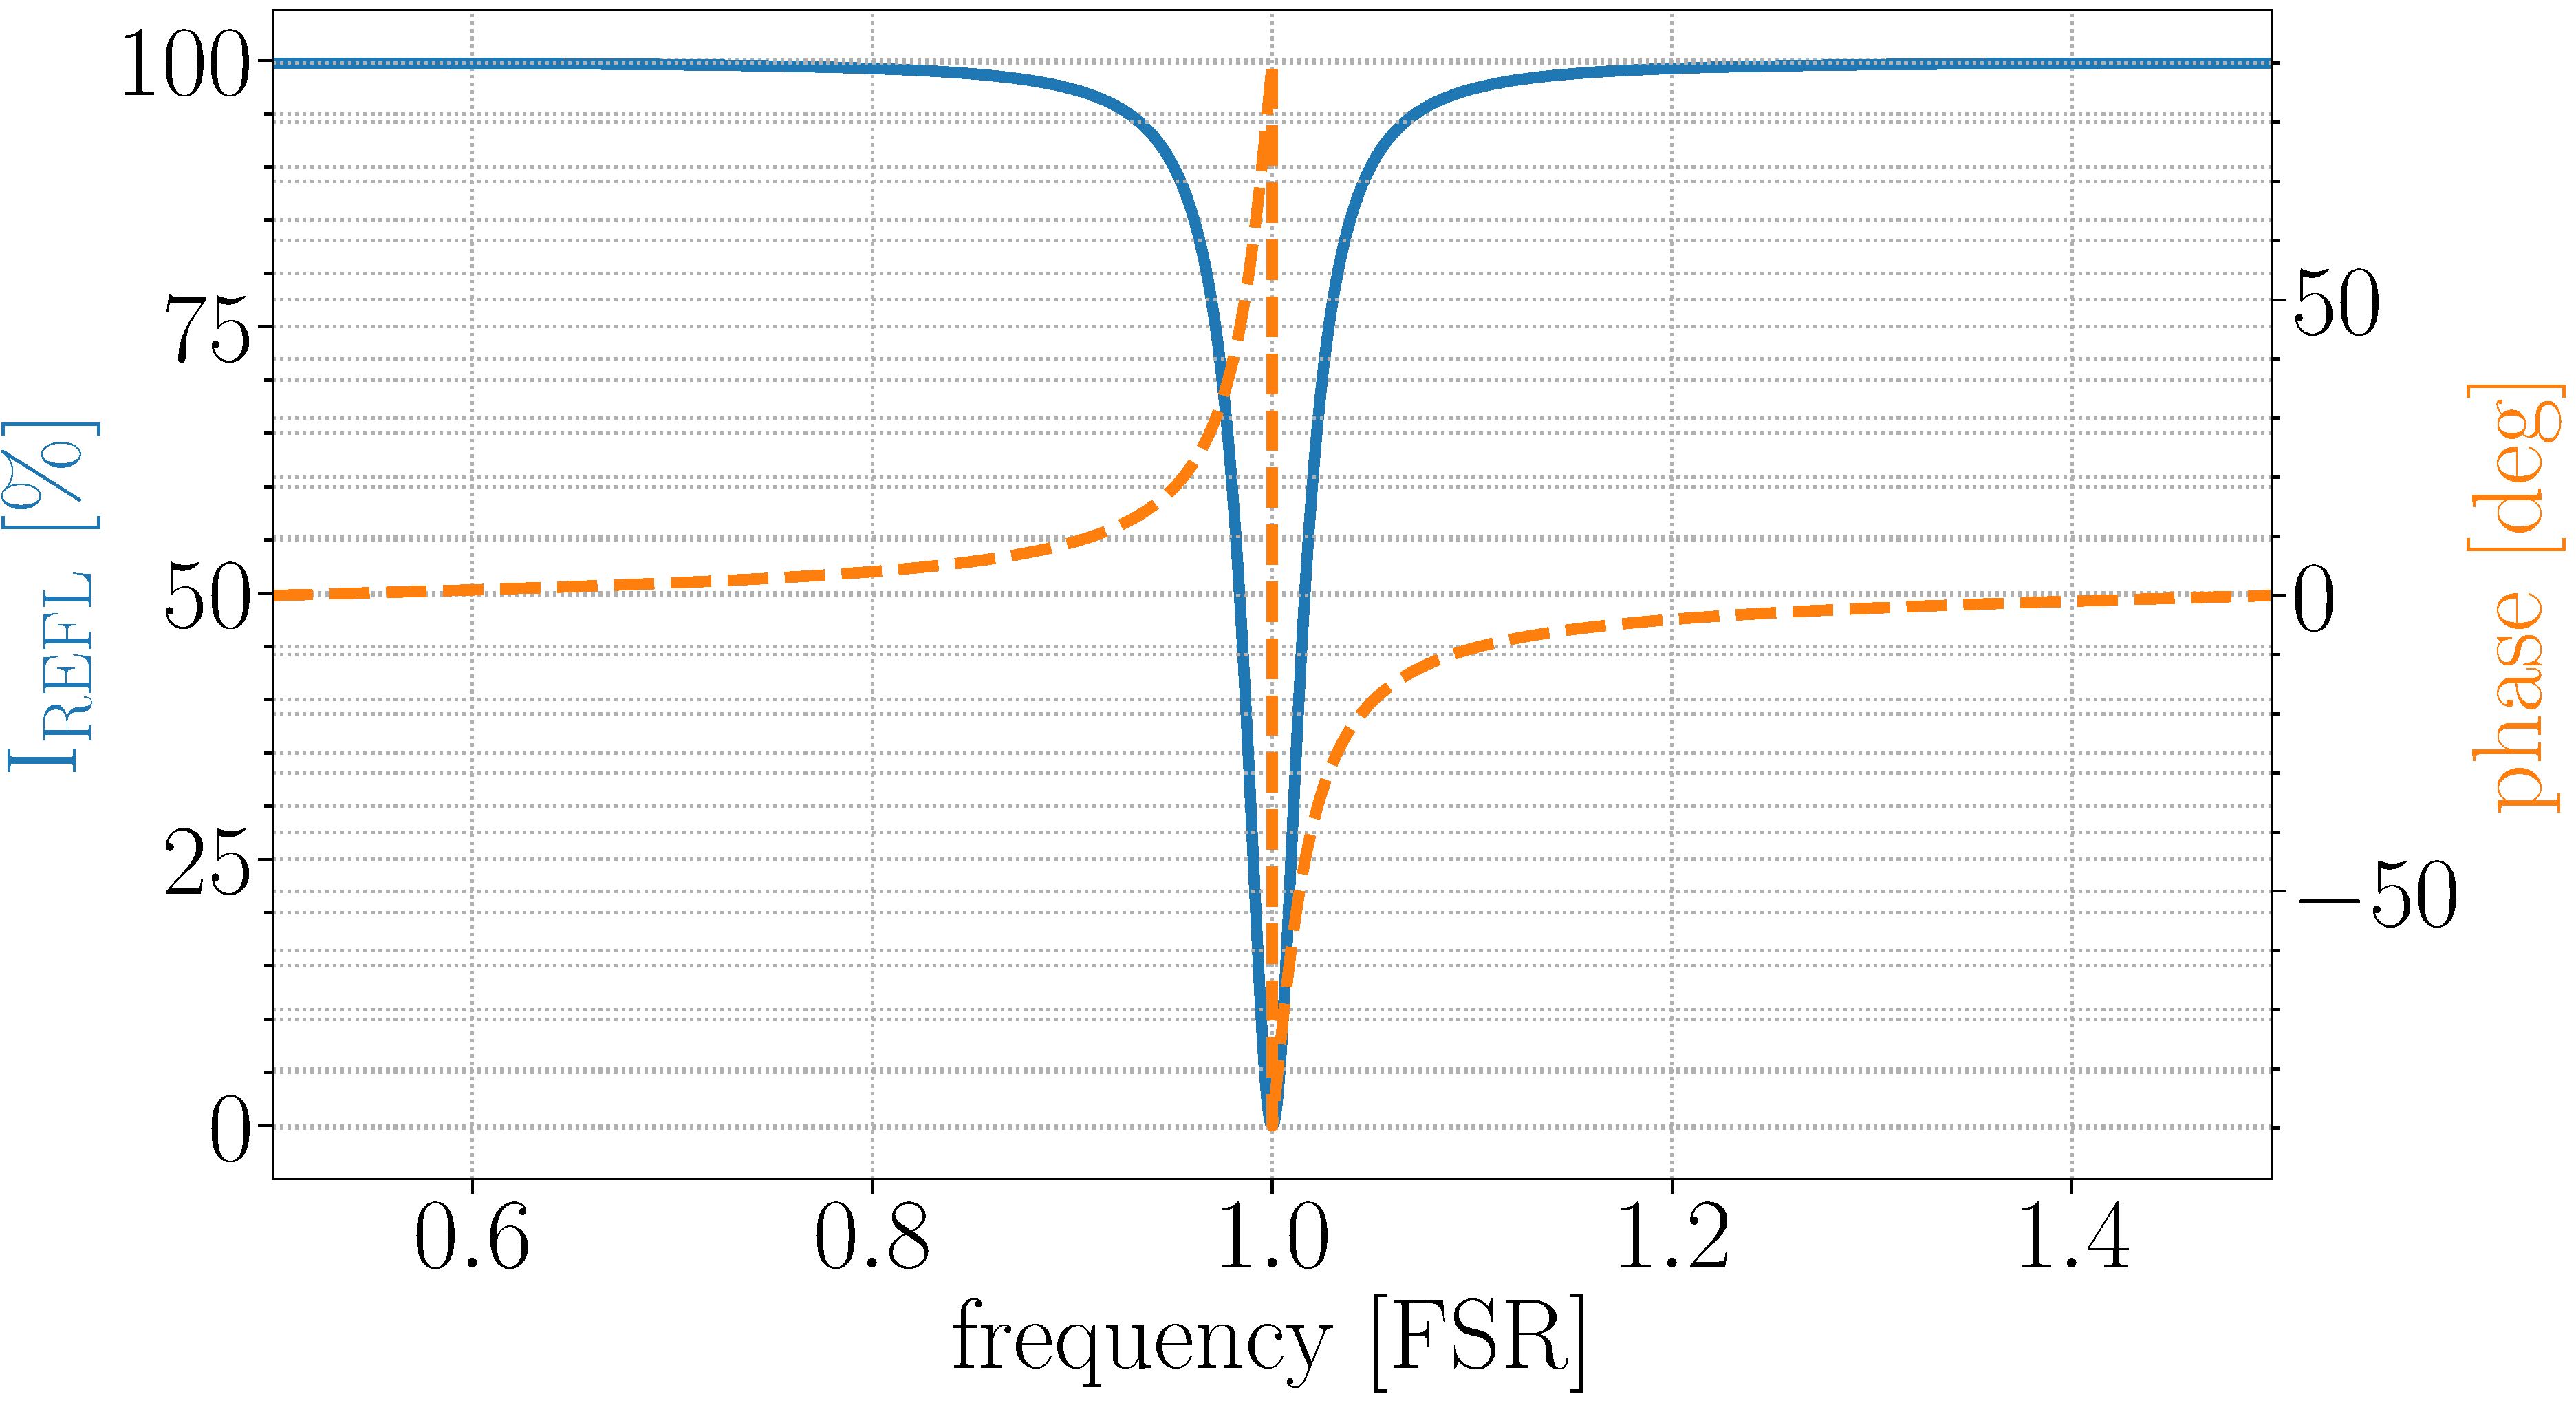
\includegraphics[width=\textwidth]{ALGAAS/REFL_cav_intensity.pdf}
\caption{Reflected cavity intensity (I$_\mathrm{REFL}$) around resonance. The resonance peak full width half maximum is set by mirror reflectivities and is succinctly quantified by the cavity \textbf{finesse} ($\mathscr{F} = \frac{\mathrm{FWHM}_\mathrm{res}}{f_\mathrm{FSR}} = \frac{\pi \sqrt{r_1 r_2}}{1-r_1 r_2}$).}
\label{fig:cav_length_response_DCpow}
\end{figure}

The ratio of the circulating power to the cavity input power is set by the reflectivity paramters of the cavity mirrors; demonstrating the coorelation to how long a given phasefront can remain stored between said mirrors at resonance. This ``cavity storage time" ($\tau_s \appropto L r_1 r_2$) translates as a length elongation with the phasefront travel history encoded in the arrival time of its photons back at the beam splitter.

\subsubsubsection{Gaussian beam phasefronts}
Imposing a Gaussian beam to our theoretical two mirror cavity and after considering \ref{eq:gaussiana careful consideration: containing the power of a diverging phasefront between two finite sized mirrors. The resonance of a gaussian beam requires, one or both of the cavity mirrors to have a finite radius of curvature to match a resonant beam's phasefront \textcolor{red}{see stability criteria}. Though alongside the TEM00 fundamental mode, the paraxial equation (\textcolor{red}{see appendix}) has families of solutions that exist for the aforementioned cavity configuration; these solutions best described by the Hermite-Gauss and Laguerre-Gauss bases:

\begin{equation}
	E_\mathrm{HG} = 
\end{equation}


\begin{equation}
	E_\mathrm{LG} = 
\end{equation}

\textcolor{red}{FIGURE: Various mode wavefront solutions with the following caption: ''The various wavefront geometries of the Hermite-Gauss [left] and Laguerre-Gauss modes [right]. Some of these modes are commonly used as error signals used for quantifying the presence of mirror misalignment and mode mismatch."}

If it wasn't clear yet, it certainly will be understood that the delicate state of cavity resonance is one that is hard to maintain and easily broken.  

\subsubsubsection{``Arm elongation''}

An intuitive analogue of the Fabry-P\'{e}rot's arm elongation capabilities can be drawn out when comparing against the Delay Line storage time~\cite{saulson2017}:

\begin{equation}
	\tau_s = \frac{L}{c} \frac{r_1r_2}{1-r_1r_2} = \frac{1}{4 \pi \mathscr{F}}
\end{equation}

Advanced LIGO, with its 4km length and approximate finesse of 208 coorelates to a storage time of $382\mu s$, whereas the simple Michelson has an arm storage time of $26 \mu s$. The cooresponding optical gain increase is noted in \ref{fig:fpmi}. 

\begin{equation}
	\mathrm{H_{FPMI}} = \frac{t_1 ^2 r_2}{(t_1^2 + r_1^2)r_2 - r_1} \frac{\mathrm{H_{MICH}}}{1 - r_1 r_2 e^{-2i \omega L / c}}
\end{equation}

\begin{figure}[ht!]
  \begin{subcaptiongroup}{\includegraphics[width=.45\textwidth,page=3]{INTRO/ifo_configs.pdf}}
  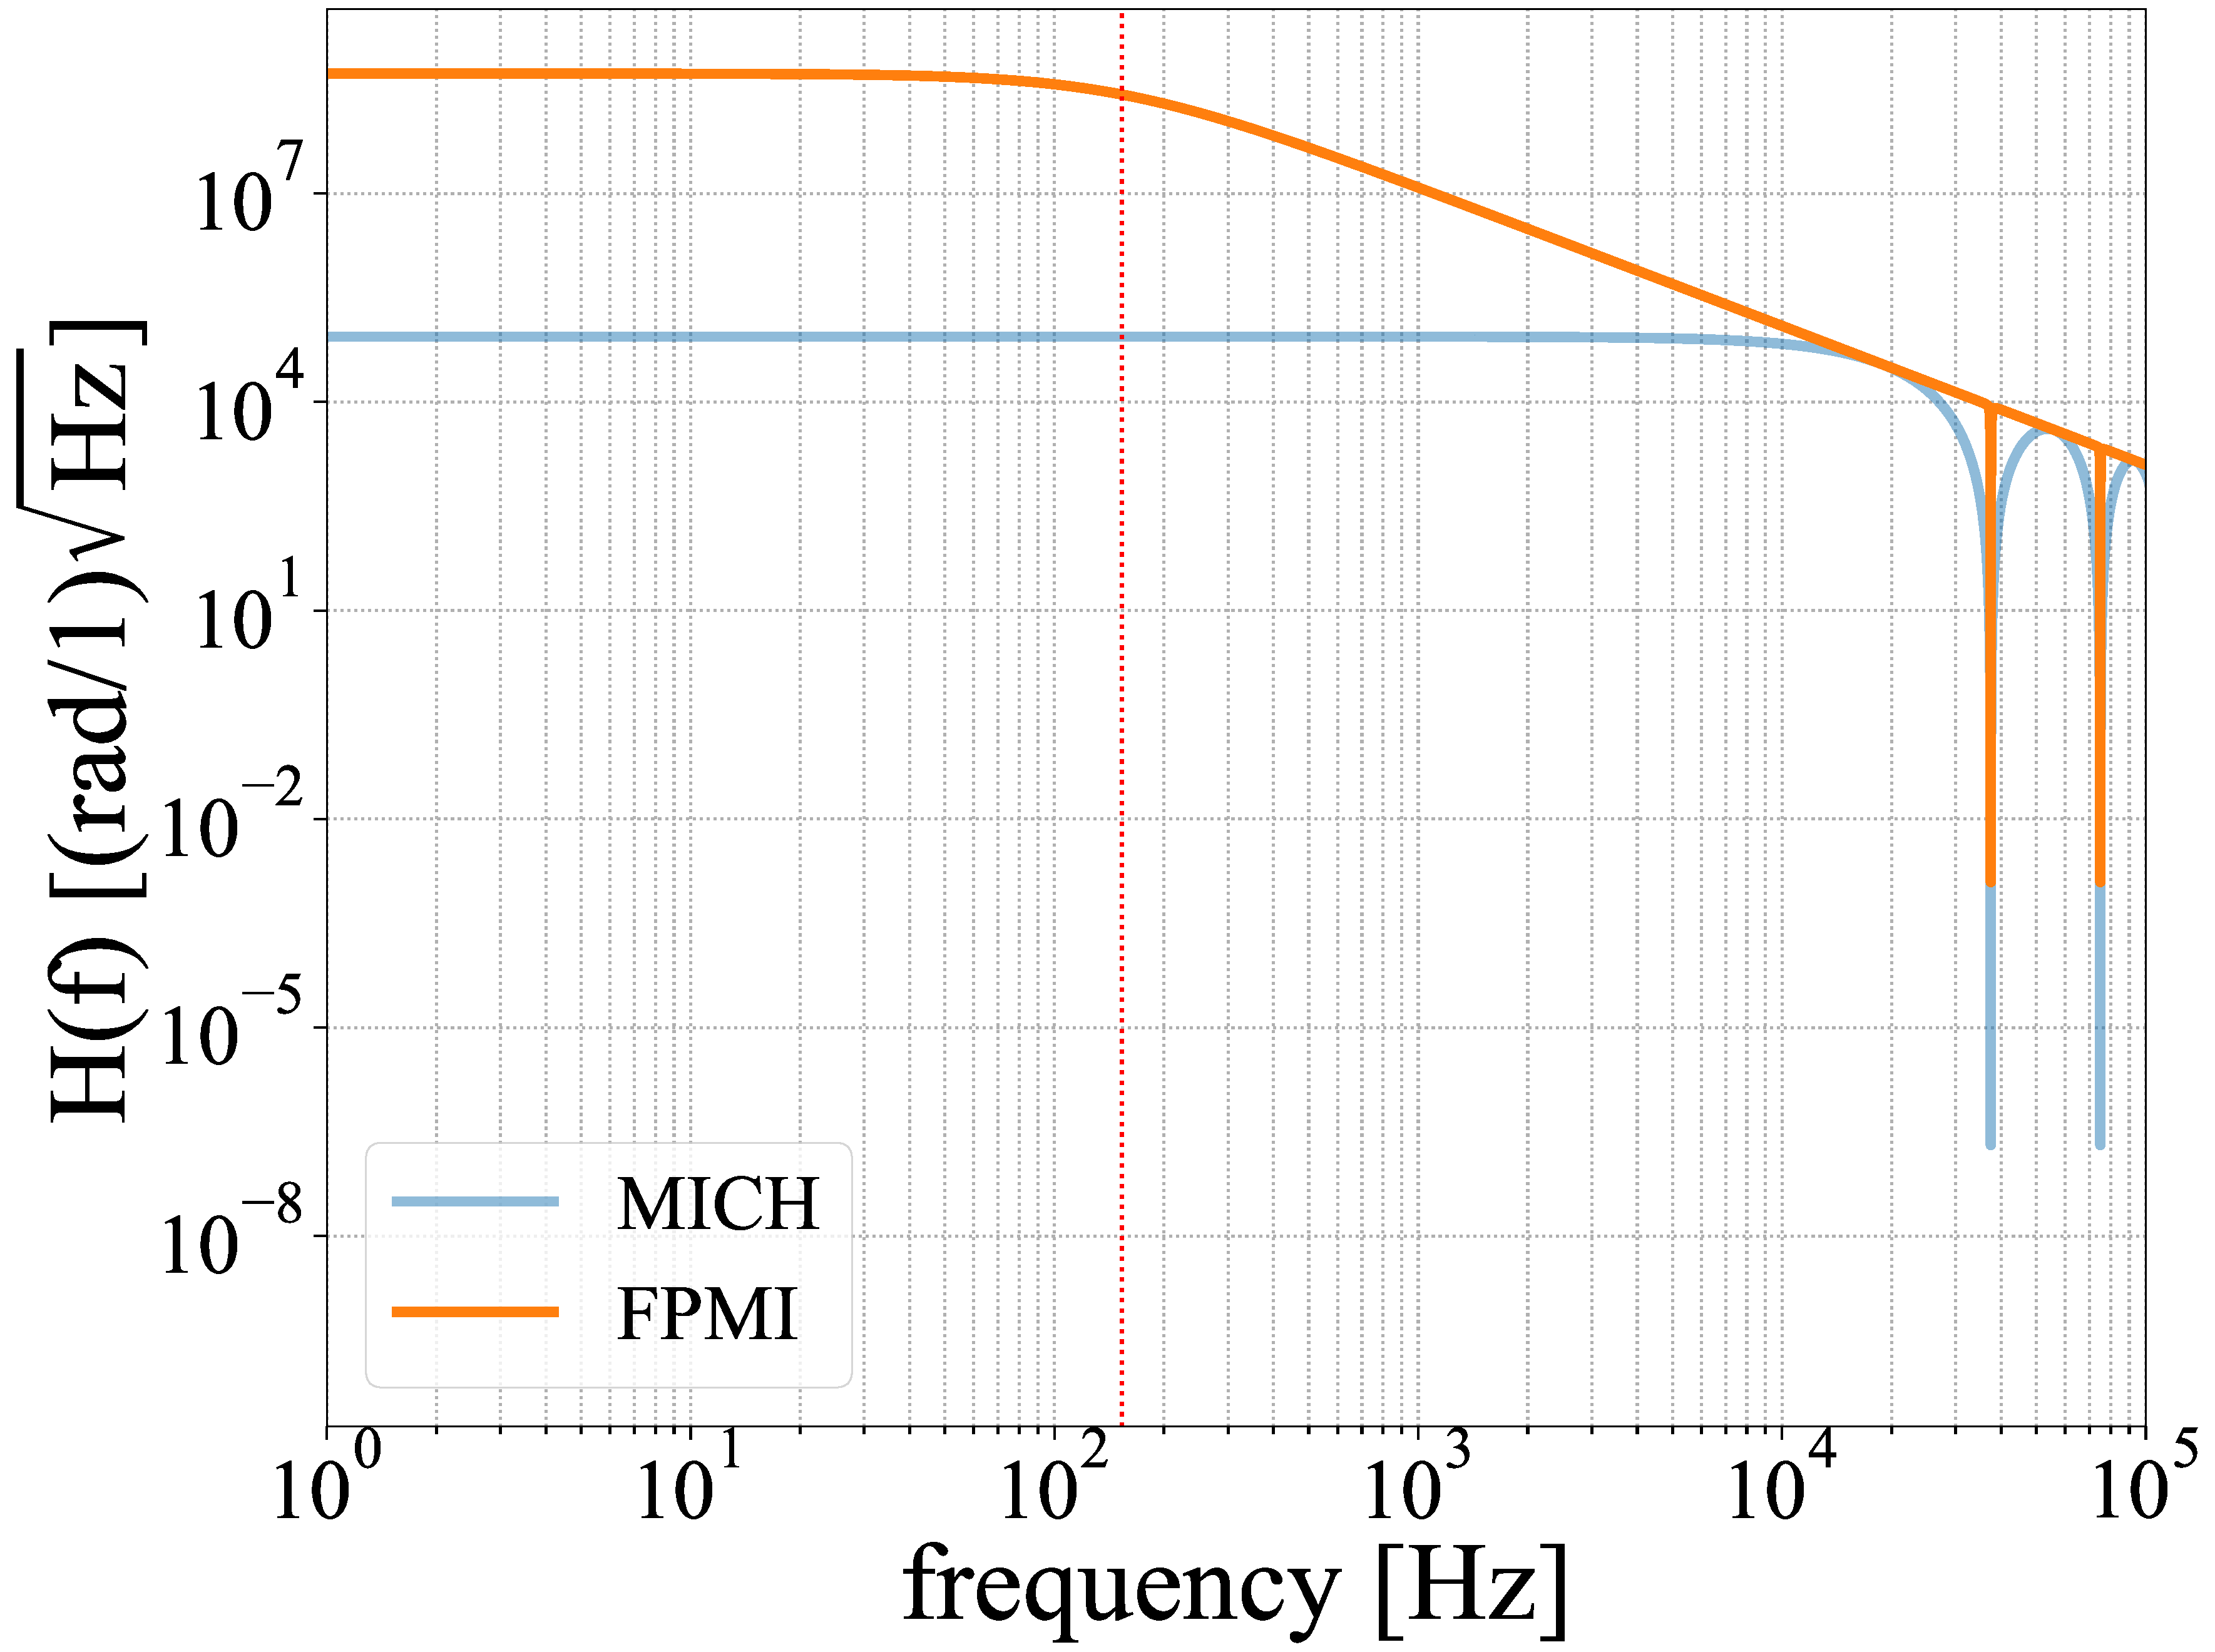
\includegraphics[width=.575\textwidth]{INTRO/fpmi_fr.pdf}
  \end{subcaptiongroup}
  \hfill
  \caption{[Left] The Fabry-P\'{e}rot Michelson optical schema and [Right] an associated optical gain.}
  \label{fig:fpmi}
\end{figure}

It's incredible that in theory adding two mirrors can present such a detector gain improvement. Though in practice this doesn't occur without: 1) maintaining fixed mirror positions within a fraction of the wavelength of the light used and 2) the reduction in detector bandwidth. In spite of this, clever experimental techniques like the Pound-Drever-Hall technique allow experimentalists to maintain these conditions ~\cite{?}.

\subsection{Dual-Recycled Fabry-Perot Michelson (DRFPMI)}
Recycling mirrors are an extension of the FPMI that exploits otherwise wasted optical power by providing a means of enhancing the optical gain and bandwidth of the instrument. Strategic tuning of mirror coating parameters and positions at symmetric and anti-symmetric ports can incorporate power recycling and signal recycling respectively.

\begin{figure}[H]
\begin{center}
\includegraphics[width=\textwidth,page=4]{INTRO/ifo_configs.pdf}
\end{center}
\caption{A simplified Dual-Recycled Fabry-Perot Michelson optical schema}
\label{fig:drfp_michelson}
\end{figure}

\subsubsection{Power Recycling}
When operating a FPMI at a dark fringe, a significant amount of power is reflected back to the symmetric port as mentioned in~\ref{section:FPC} leading to the consistent waste of optical power if simply dumped. Placing an additional highly reflective mirror at the symmetric port and while maintaining resonance of the carrier to the arms, you can reintroduce (or ``recycle") power back to the arm cavities. A PDH loop is utilized for carrier resonance, and the macroscopic positioning of the PRM is informed by the choice of optical sideband frequency required when applying PDH. 

\begin{equation}
	\mathrm{G_{PR}} = \frac{(1-r_\mathrm{PRM}^2)}{1-r_\mathrm{PRM}[1- (\mathscr{F} \mathscr{L}_\mathrm{RT})/ \pi]}
\end{equation}

With a maximum recycling gain \ref{}: 

\begin{equation}
	\mathrm{G_{PR}} = \frac{\pi}{2 \mathscr{F} \mathscr{L}_\mathrm{RT}} \bigg[ \frac{1}{1- \frac{ \mathscr{F} \mathscr{L}_\mathrm{RT}}{ 2 \pi}} \bigg]
\end{equation}

\subsubsection{Signal Recycling}
As may be implied, the technique requires a mirror installation at the anti-symmetric port; though with a more nuianced approach than that of power recycling. By simply placing a partially reflective mirror at the output port it is understood that light leakage coming from the PRFPMI at the anti-symmetric port (caused by differential arm motion) is re-introduced to the arms. The signal recycling mirror reflectivity cannot be set too high to avoid attenuation to the PRFPMI output. Though the detector enhancement only comes after exacting the cost of trading off the detector bandwidth for increased detector gain and vice versa. The operating point between the maxima of these two detection characteristics is a function of the microscopic length (phase) tuning:

\begin{equation}
	\mathrm{H}_\mathrm{DRFPMI} = \mathrm{G}_\mathrm{PR} \mathrm{P}_\mathrm{in} L \Omega \bigg[ \frac{ t_\mathrm{ITM}^2 r_\mathrm{ETM}}{(t_\mathrm{ITM}^2 + r_\mathrm{ITM}^2)r_\mathrm{ETM} - r_\mathrm{ITM}}  t_\mathrm{SRC} \frac{e^{-i 2 \pi L f / c} \mathrm{sin}( 2 \pi f / c)}{ 2 \pi L f } \frac{\mathrm{sin}(\phi_0)}{1- r_\mathrm{SRC}r_\mathrm{ETM} e^{-i 4 \pi L f / c}} \bigg]
\end{equation}

\begin{equation}
\begin{align}
	t_\mathm{SRC} & = \frac{t_\mathrm{SRM} t_\mathrm{ITM} e^{i\phi_\mathrm{SRC}}}{1-r_\mathrm{ITM} r_\mathrm{SRM} e^{i2\phi_\mathrm{SRC}}}, \\
	r_\mathrm{SRC} & = \frac{r_\mathrm{ITM} - r_\mathrm{SRM} e^{i2\phi_\mathrm{SRC}}}{1-r_\mathrm{ITM} r_\mathrm{SRM} e^{i2\phi_\mathrm{SRC}}} \\
\end{align}
\end{equation}

\begin{figure}[H]
  \begin{subcaptiongroup}
	  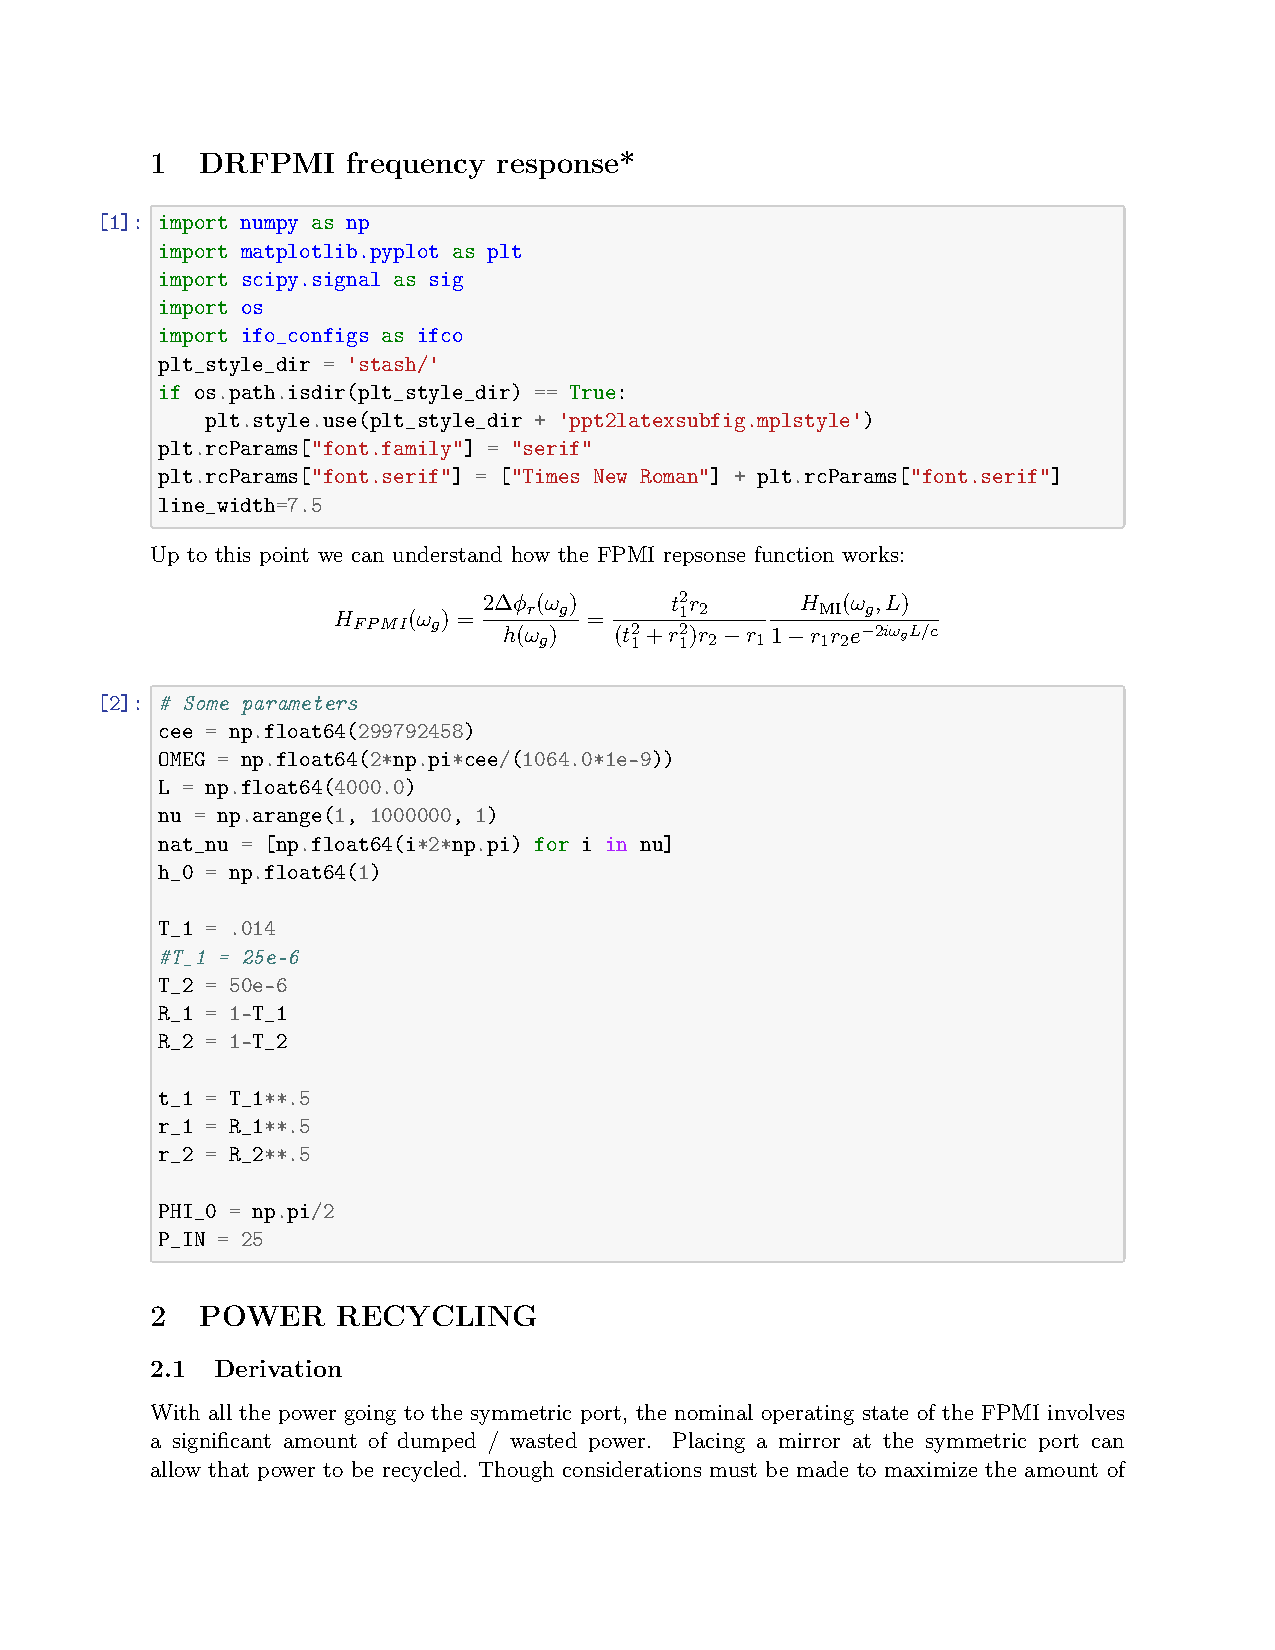
\includegraphics[width=.487\textwidth]{INTRO/drfpmi_fr.pdf}
 	  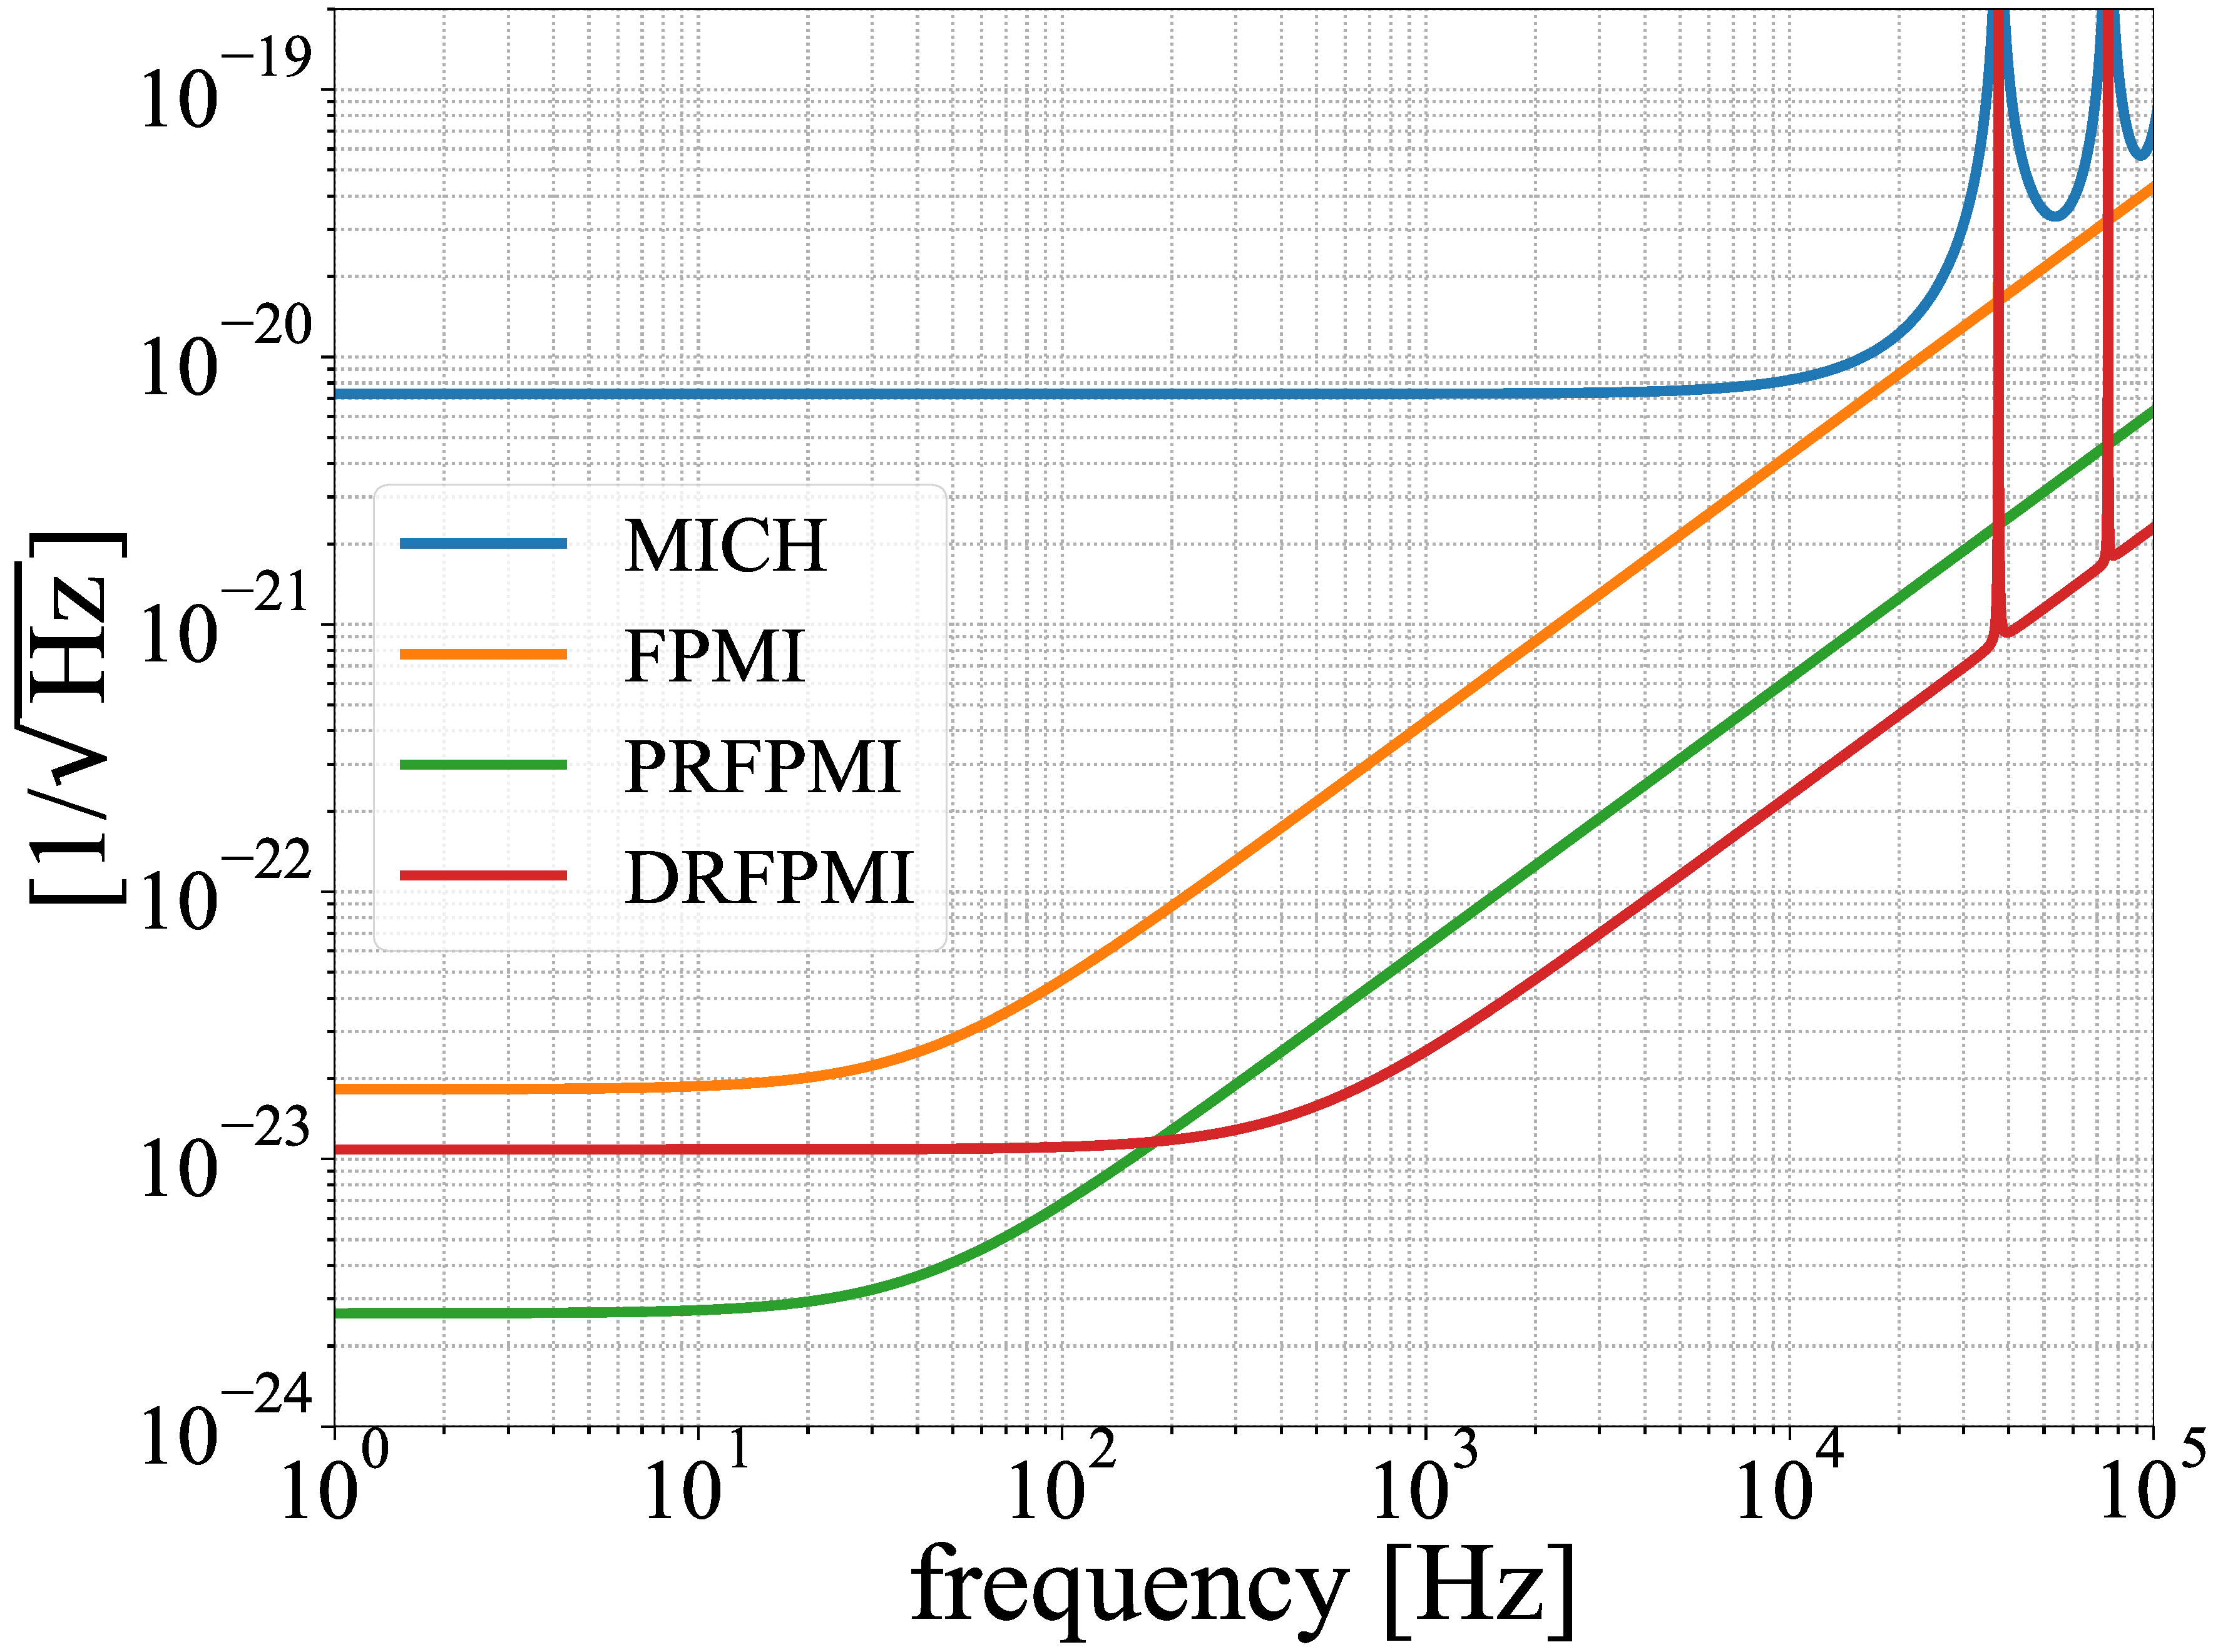
\includegraphics[width=.5\textwidth]{INTRO/strain_compare.pdf}
  \end{subcaptiongroup}
  \hfill
  \caption{[Left] Comparison of all optical gain functions [Right] Coorelated shot nosie strain sensitivity.}
  \label{fig:drfpmi_gain_and_strain}
\end{figure}

\section{ALIGO}

\begin{figure}[H]
  \begin{center}
	  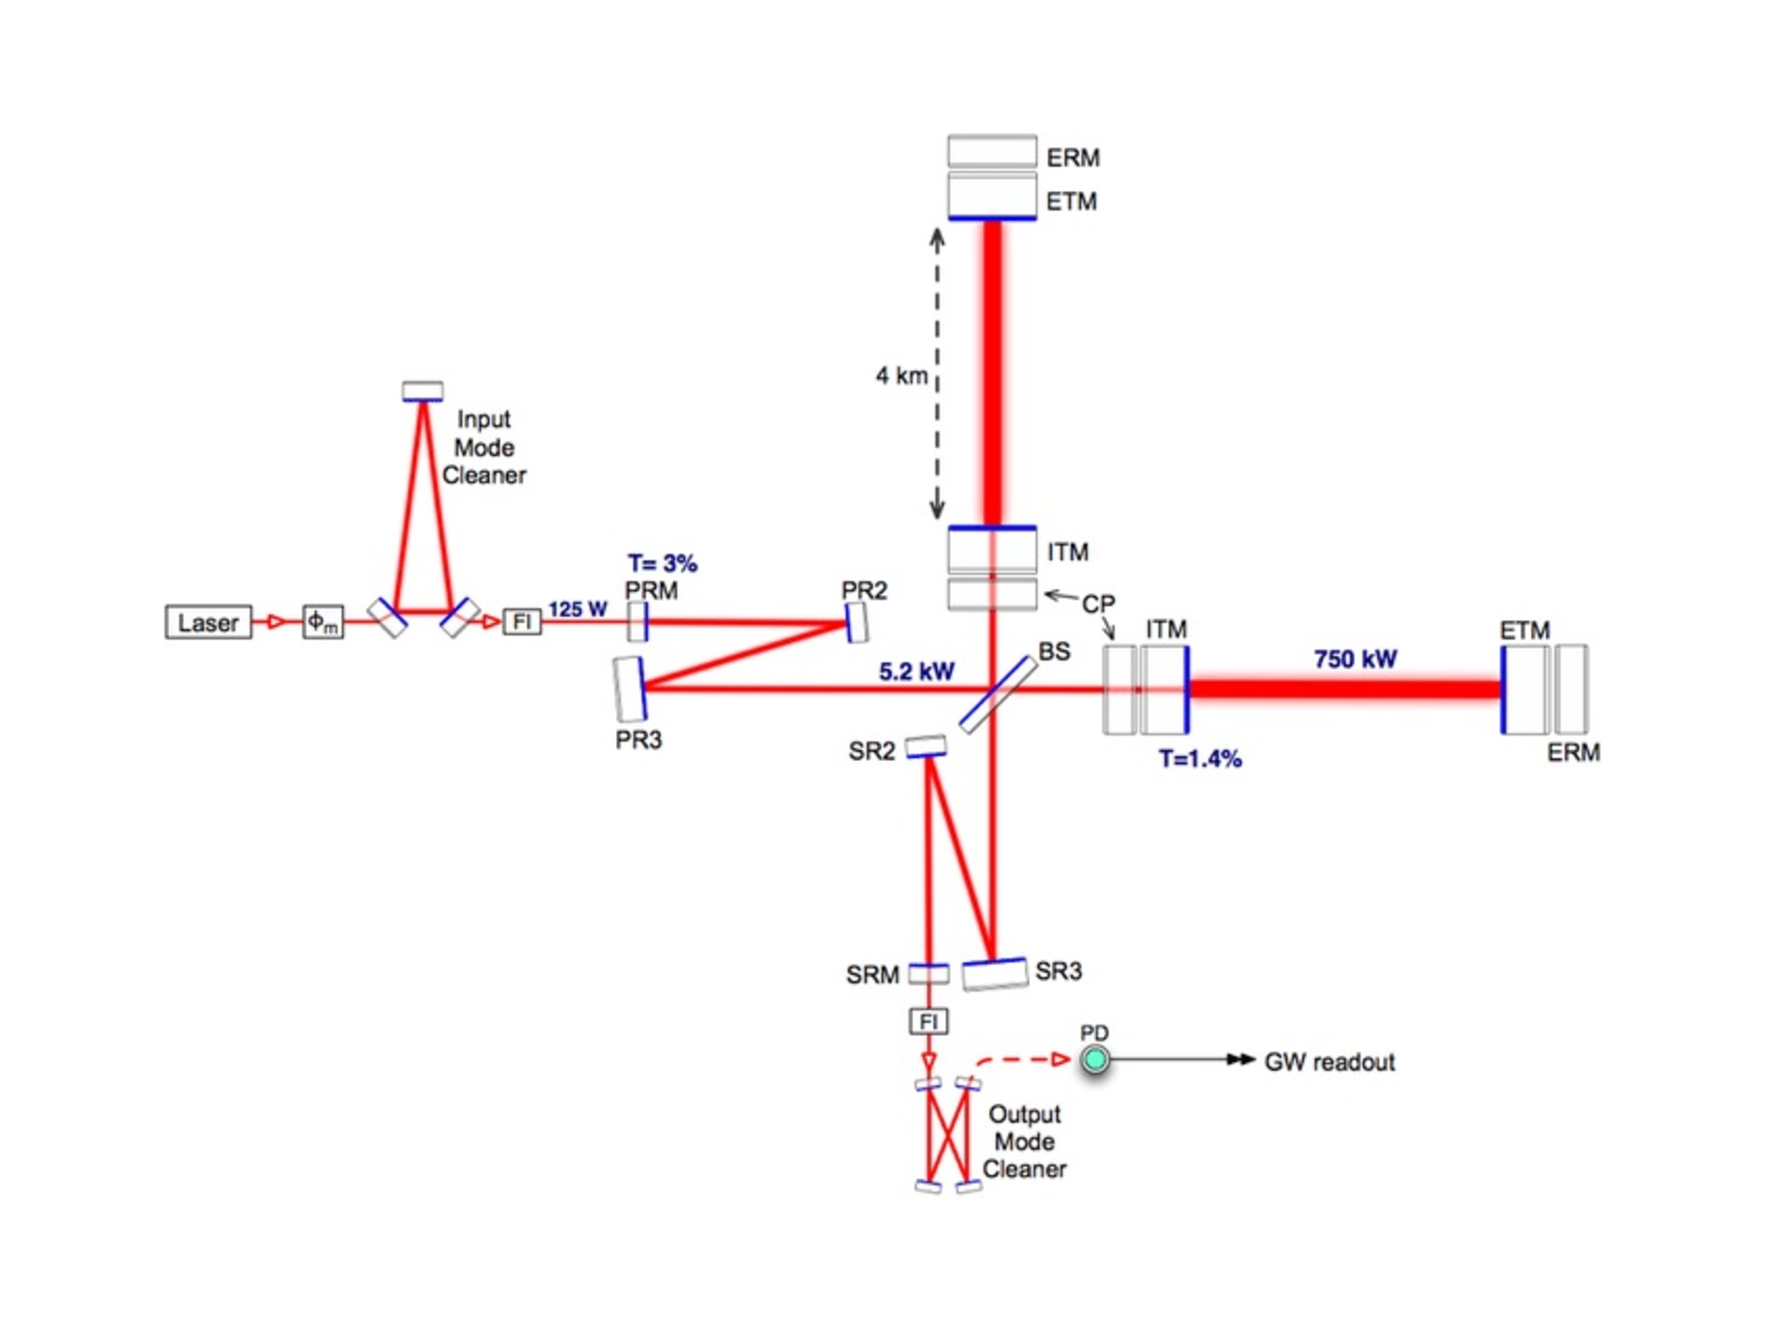
\includegraphics[width=\textwidth]{aligo_config.pdf}
  \end{center}
  \caption{DRFPMI configuration used in ALIGO}
  \label{fig:simple_michelson}
\end{figure}

``Core optics" (Recycling mirrors, Beam splitter, and FP arm cavity mirrors) are suspended with quadruple pendulum suspensions decoupling seismic activity from the mirror positions to as low as a frequency as possible. 

\subsection{Reaching ``Observing Mode"}
The prior discussions still have yet to discuss most of the practical considerations that are required to operate a DRFPMI as a gravitational wave observatory. For the sake of narrowing down the relevance to the body of this work, we discuss more subtle features of the detector: one requires some knowledge of beam optics while the other involves the thermodynamic noise limitation of highly reflective mirror coatings. Alongside this, it is important to know that the studies take place at two very different stages of detector comissoning (One is aimed at comissioning current detectors and the other aims at informing choices to be made for next generation detectors) though both are aimed at increasing gravitational wave detector sensitivity.  The current objective at hand is to inform of these essential criteria for interferometer operations as they pertain to this dissertation. More details on setting up the simple Michelson provides on some of the initial requirements; while the second order is establishing the strict conditions of the Fabry-P\'{e}rot cavities.


\subsubsection{Length Stabilization}
With LIGO's coupled cavity configuration, maintaining mirror positions is imperative. Techniques such as the offset lock (using a DC photodiode to measure the transmitted, reflected, or circulating power within a linear and slightly off resonance point) \cite{} and the Pound-Drever-Hall technique (see \ref{subsubsec:pdh} ) are used to maintain cavity length stabilization. Stabilizing cavity lengths to configure the detector into a highly sensitive differential arm sensor is a process that is worthwhile understanding with more ample discussions ~\cite{Mullavey:12}.


So far, we've discussed light and phase fronts without addressing geometric constraints when using Gaussian laser light. We consider a general complex Gaussian beam mode propogating along the beam axis ($z$) with wavelength $\lambda$.

\begin{equation}\label{eq:gaussian_beam}
E(r) = E_o \frac{\sqrt{[\lambda z_o] / \pi}}{W(z)}e^{-r^2 / W^2(z)} e^{-ikz - ik[r^2 / (2R(z))] + i \zeta}
\end{equation}

Where $E_o$ is a complex amplitude, $r = \sqrt{x^2 + y^2}$ defines the transverse beam coordinates, $k$ is the wave number, $W(z)$ is the beam width, $R(z)$ is the beam radius of curvature, and $\zeta$ is the Gouy phase.

Derived from the paraxial approximation of the Helmholtz equation, this field is not the only solution for optical cavities. Alternative higher order mode (HOM) solutions are commonly present and are expressed in terms of two mathematical bases: the Hermite-Gauss and Laguerre-Gauss modes. These HOMs are more often than not power parasites when attempting to only sense displacement Fabry-P\'{e}rot cavities and are a symptom of altered cavity geometry; though a virtue of the lost power is its utility as an error signal for sensing and actuation schemes. This is what is what is accomplished with an alignment sensing and control (ASC) system and a thermal compensation system (TCS) for mode matching actuation.

\textcolor{red}{FIGURE: ALIGO Sensor and Actuation schema?}

\subsubsection{Alignment sensing and control}

\begin{figure}[H]
    \begin{center}
    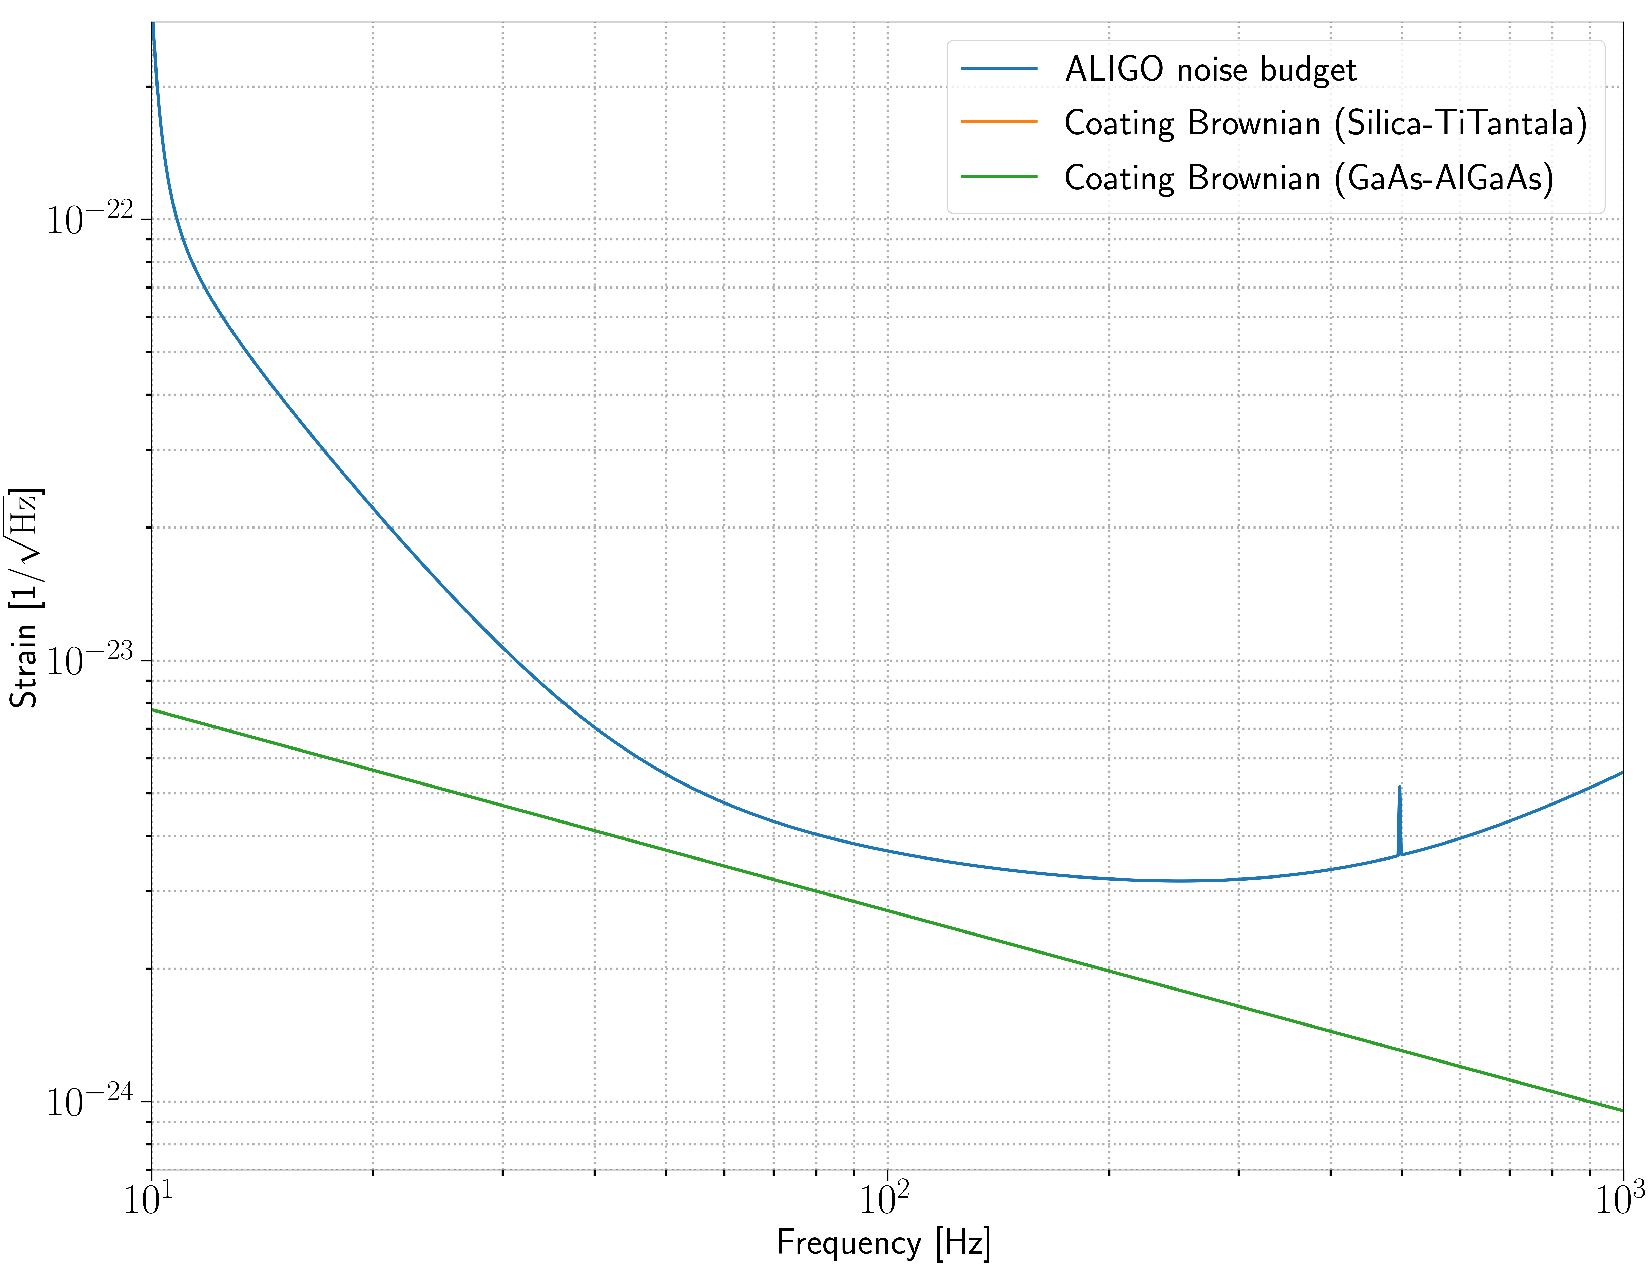
\includegraphics[width=.5\textwidth]{ALGAAS/aligo_nb_plus_cbn.pdf}
    \end{center}
    \caption{A misaligned Fabry-P\'{e}rot cavity scatters circulating light into higher order Hermite-Gauss modes.}
\label{fig:aligo_tn_comparison}
\end{figure}

\begin{equation}
	E_{n,m}(x,y,z) = E_o \bigg[ \frac{W_o}{W(z)} \bigg] H_n \bigg[ \frac{\sqrt{2}x}{W(z)} \bigg] H_m \bigg[ \frac{\sqrt{2}x}{W(z)} \bigg] e^{-(x^2 + y^2)/W(z) - ikz - ik[(x^2 + y^2)/(2R(z))] + i(n + m + 1)\zeta(z)}
\end{equation}

Even with state-of-the-art ground motion isolation for terrestrial gravitational detectors using quadruple stage pendula and high mass mirrors, current gravitational wave detectors still suffer from occasional misalignment and require sensing and feedback loops to meet mirror alignment requirements.

\subsubsection{Mode Matching}
For Gaussian beams, there are further requirements of macroscopic mirror positions and radius of curvatures to maximize resonant power in the fundamental (TEM00) mode. Failure to plan and maintain these conditions sucessfully results in a mismatch of the beam mode to the cavity mode, scattering power into higher order Laguerre-Gauss modes.  

\begin{equation}
	E_{n,m}(\rho, \phi, z) =  E_o \bigg[ \frac{W_o}{W(z)} \bigg] H_n \bigg[ \frac{\rho}{W(z)} \bigg]^2 L^n_m \bigg[ \frac{\sqrt{2}\rho^2}{W^2(z)} \bigg] e^{-\rho^2/W(z) - ikz - ik[\rho^2/(2R(z))] - jn \phi + i(n + 2m + 1)\zeta(z)}
\end{equation}

Even with ultra-low absorption HR mirror coatings and fused silica substrates, circulating power is estimated to reach $\geq$ 200 kW, distorting the radius of curvatures of the arm cavity mirrors by ? m; which can introduce significant optical loss due to mode mismatch (esp. for coupled cavities). And as a DRFPMI like aLIGO approaches designed sensitivity, instances of mode mismatch can be a two-fold threat with optical loss to higher order modes also impacting the ability to produced squeezed light states~\cite{}. The solution implemented in aLIGO as of O3 to sense mode mismatch consists of hartmann wavefront sensors (HWS) with 800 nm and 833 nm probe beams providing real-time mirror lensing / surface distortion data while actuation comes in the form of induced thermal actuation on mirrors throughout the interferometers with particular focus on the arm cavity mirrors. The thermal actuation of the core optics comes in two varieties: a CO2 laser actuator impinging upon a pre-installed fused silica compensation plate (CP) for positive lens actuation and an annular ring heater for negative lens actuation \cite{}. 

\begin{figure}[H]
	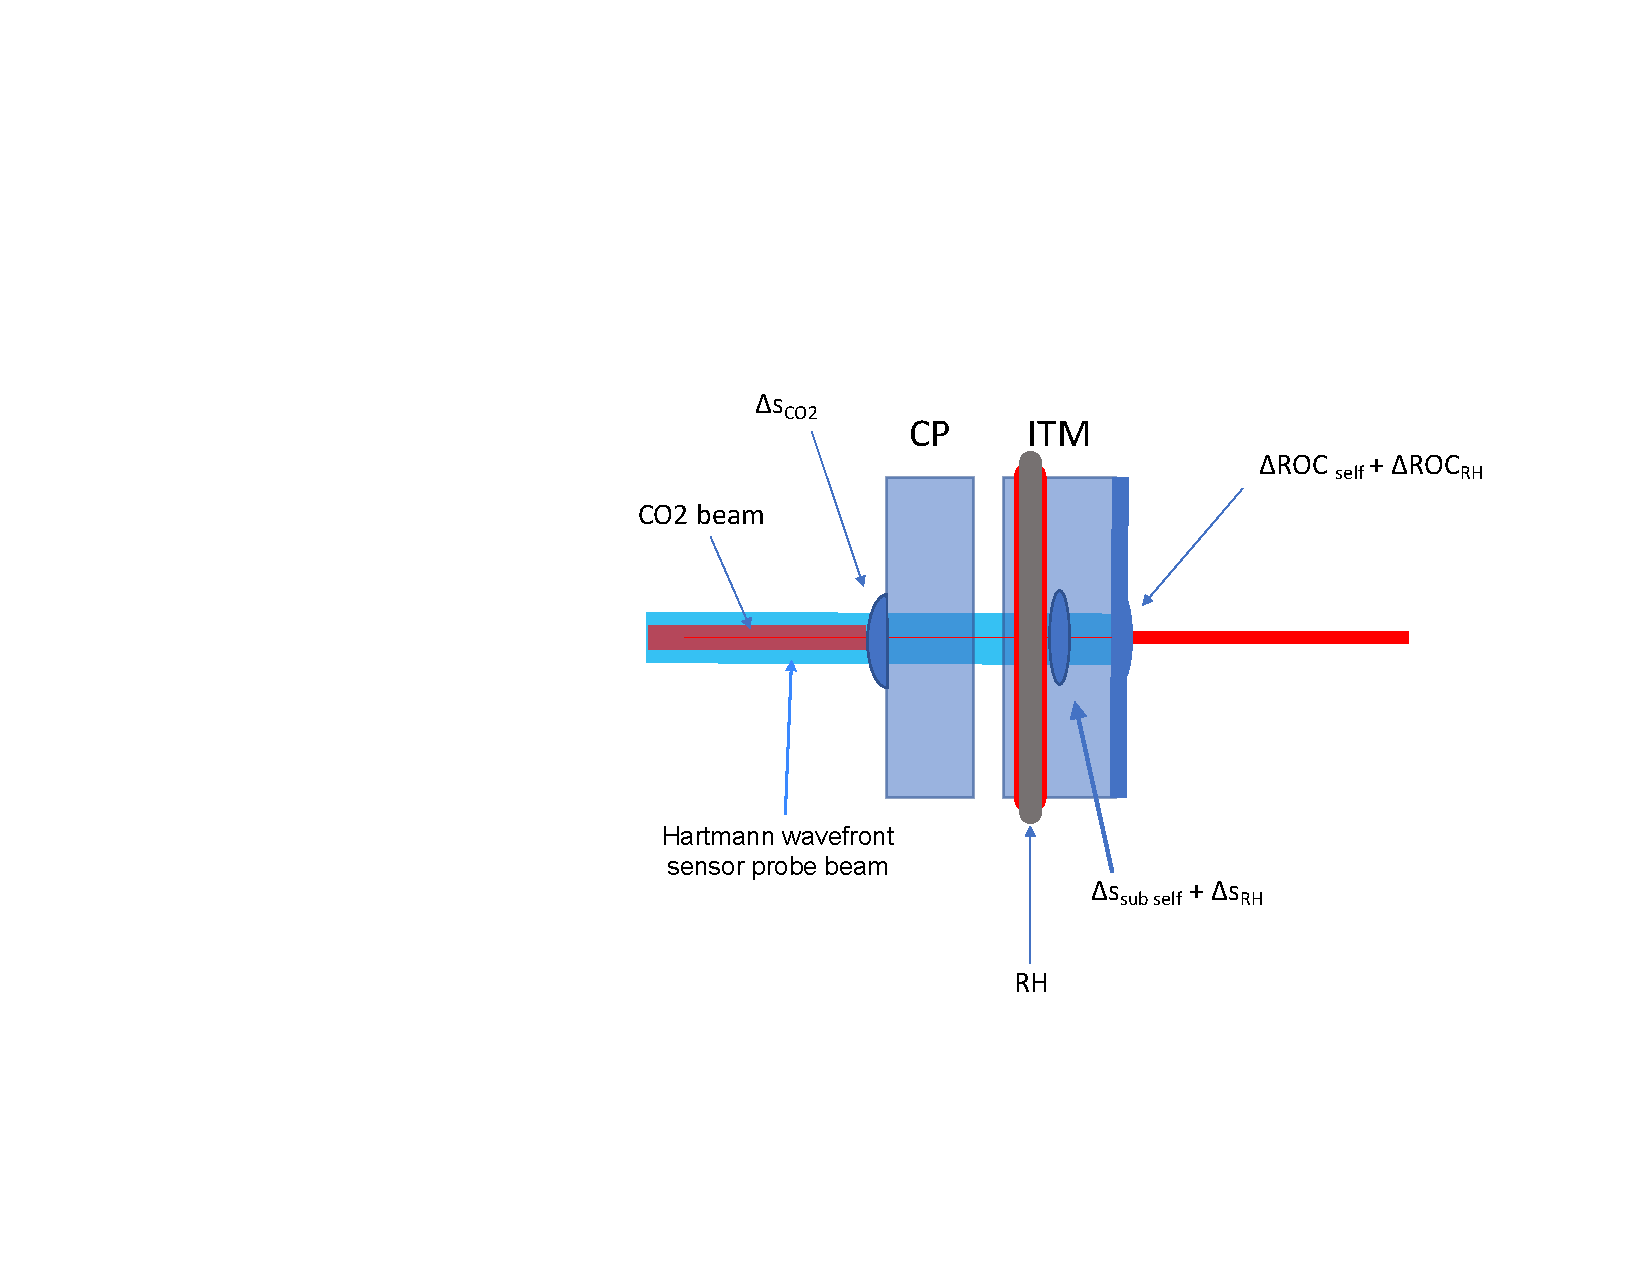
\includegraphics[width=\textwidth]{TCS/FP_input_coupler.pdf}
\caption{Thermal compensation at a single Fabry-P\'{e}rot input mirror coupler for ALIGO.}
 \label{fig:meas}
\end{figure}

\section{Detector Noise}

\section{Coating Thermal Noise}
Contributions of categorized noises for gravitational wave detectors are organized in a ''noise budget", comprised of a collection of technical (noise imposed by the practical operation of the detector) and fundamental (inherent physical limitations of DRFPMIs by design) noise sources that impose limitations on gravitational wave detection.
\textcolor{red}{Contributions of categorized noises for gravitational wave detectors the ''noise budget" ((LHO and LLO O3?) or just GWINC?)}

\subsection{Brownian Thermal Noise}
\textcolor{red}{Might move this section back to the $\algaas$ Electro-optic noise chapter}
\\
In 1827 the Scottish botanist Robert Brown noticed a constant motion of pollen particulates on the surface of water; witnessing randomized collisions of the water molecules holding a kinetic energy proportional to the temperature ($k_BT$) \cite{Brown:1828}. It is because of his documented observations we name the phenomena Brownian motion. And although the observations were on motion of particulates in liquids, molecules and atoms within gases and solids also exhibit Brownian motion. For high precision optical experiments operating at room temperature (and higher due to high power resonant beams), understanding how much differential phase noise is imparted on the interferometer light passing through and reflecting from core optics is crucial. This requires knowledge of the mean squared displacement from each degree of freedom of the system which can be realized through the Fluctuation Dissapation theorem. Derived by H.B. Callen and T.A. Welton, the theorem states that for a randomly fluctuating linear force \cite{Callen:1951}:

 %% Further insight into Brownian motion was explored by Einstein where he was able to relate the mean-square displacement of a particle of radius $r_\mathrm{sph}$ on a fluid with viscosity $\eta$.

 %%\begin{equation}
 %%\overline{x^2} = k_B T  \frac{1}{3 \pi \eta  r_\mathrm{sph}}
 %%\end{equation}

 %%This relation has important implications about how the random motion or fluctuations of a particulate (the pollen) is influenced (dissipated) by the viscosity of the surrounding medium (water).

\begin{equation}
F_x^2(f) = 4 k_B T\; \Re[Z]
\end{equation}

 \noindent Where $\Re[Z]$ is the real part of the impedance of the system. This impedance directly relates to equations of motion:

 \begin{equation}
 Z = \frac{F}{\dot{x}}
 \end{equation}

\noindent Another useful form is the power spectrum of the fluctuating motion:
\begin{equation}\label{fdtpsd}
x^2 (f)  = \frac{4k_B T}{(2 \pi f)^2}\; \Re[Y]
\end{equation}

Where $Y$ is the inverse of the impedance or admittance. With this power spectra, modelling and budgeting notable LIGO fundamental noise contributions attributed to the choice of the materials used for mirror substrates, and highly reflective mirror coatings becomes less daunting. Though adequate modelling of internal force couplings for the aforementioned components is required.

\subsubsection{Internal friction in Materials and Loss angle}

Zener provides a model of the internal friction of materials incorporating anelasticity into the equations of motion \cite{zener:1948}:

\begin{equation}
F = k(1+i\phi)x + m\ddot{x}
\end{equation}


Where $m$ is mass attached to a spring with a spring constant $k(1+ i\phi)$ incorporating the degree of anelasticity $\phi$. From equations 3.5 and 3.3 we perform a Laplace transform and acquire the following form of admittance:
\begin{equation}
Y(s) = \frac{\dot{x}(s)}{F(s)} = \frac{-s}{k(1+i\phi) + ms^2}
\end{equation}

\noindent Or more transparently the Fourier representation since we assume a linear time invariant system:

\begin{equation}\label{admitint}
Y(\omega) = \frac{\dot{x}(\omega)}{F(\omega)} = \frac{-i\omega}{k(1+i\phi) - m\omega^2} = \frac{k \omega \phi - i \omega (k - m \omega^2)}{(k-m\omega^2)^2 +k^2 \phi^2}
\end{equation}

\noindent Plugging equation \ref{admitint} back into \ref{fdtpsd}:

\begin{equation}
x^2 (f)  = \frac{2k_B T}{\pi}\frac{k\phi}{(k-4\pi^2 m f^2)^2 + k^2 \phi^2}
\end{equation}
Computing the admittance from a Gaussian beam impinging upon a HR mirror can require expansion of all individual mechanical degrees of freedom of the test mass system across a relevant frequency range, and with that approach convergence is not guaranteed. Saulson and Gonzalez provide an alternative method to computing the admittance coined the ``direct approach" by Levin when computing the noise from a Gaussian beam on a LIGO HR test mass. The admittance can be acquired through:

\begin{equation}\label{admitdirec}
\Re[Y] = \frac{W_\mathrm{diss}}{F_o^2}
\end{equation}

\noindent $W_\mathrm{diss}$ is the dissipated power from the system due to an oscillating force $F_o$. This form of the admittance reveals an important result of the fluctuation dissapation theorem where an undriven system with a dissapative actor, imparts motion to the degrees of freedom via a driving force by virtue of that same actor at finite temperatures. This direct approach also allows the surface pressure applied by the Gaussian beam to interrogate which mechanical modes of the test mass impose a significant energy when \ref{admitdirec} is plugged into \ref{fdtpsd}. In the case of the gaussian beam / uncoated test mass studied by Levin \cite{levin:1998}:

\begin{equation}
S_x(f) = \frac{4 k_B T}{f} \frac{1-\sigma^2}{\pi^3 E_o r_o} I\phi \bigg[1- O\bigg( \frac{r_o}{R} \bigg)\bigg]
\end{equation}

%this requires that the driving force used in a lab mimics that of a force from a centered Gaussian beam.

\textcolor{red}{Refer to Levin appendix for more on how elasticity parameters are introduced?} Where $\phi$ and $E_o$ are the Poisson ratio and Young's modulus respectively, and $O(\frac{r_o}{R})$ contains a correction term contribution as a function of the small beam radius ($r_o$) relative to the mirror radius ($R$).

\subsubsection{Coating Brownian thermal noise}
Further investigations into the beam/optic system utilizing this approach and elasticity theory led to a deeper understanding about Brownian thermal noise contributions from LIGO test masses (substrate, suspensions, HR coating). Levin mentions, with details from Harry, that the noise contributed by a lossy mirror coating is proven to be to be the most significant contributor of brownian thermal noise. Hong provides a power spectral density \cite{Hong:2013}:

\begin{equation}
S_j^X = \frac{4k_B T \lambda \phi_x^j(1- \sigma_j - 2 \sigma_j^2)}{3 \pi^2 f Y_j (1-\sigma_j)^2 \omega_o^2}
\end{equation}

Where X represents bulk and shear with j = odd (material 1) and j = even (material 2) alternating layers representing high and low index materials j = odd (material 1) j = even (material 2) for an HR coating.

\begin{figure}[H]
    \begin{center}
    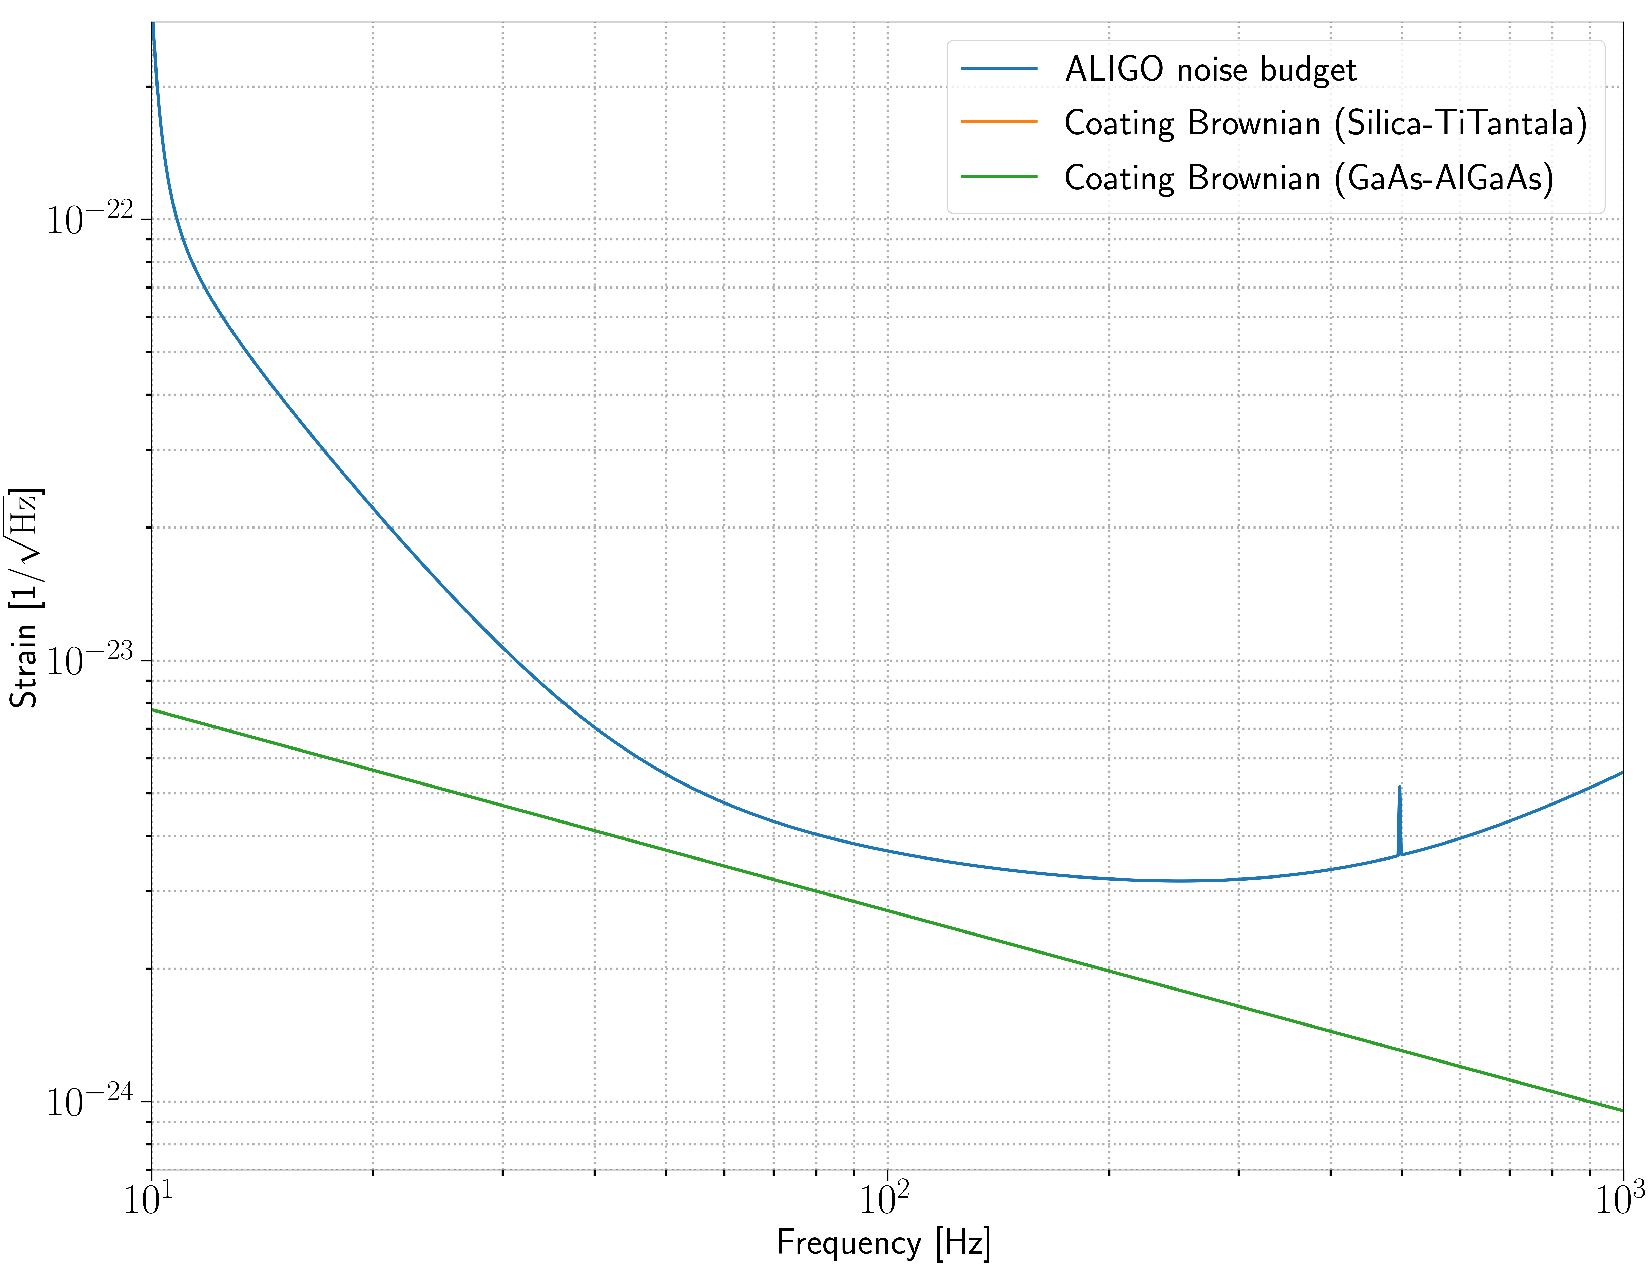
\includegraphics[width=\textwidth]{ALGAAS/aligo_nb_plus_cbn.pdf}
    \end{center}
    \caption{ALIGO noise budget placeholder for silica-tantala, and gaas-algaas brownian noise comparison}
\label{fig:aligo_tn_comparison}
\end{figure}

\subsubsection{$\mathrm{SiO_2}/\mathrm{TiO_2:Ta_2O_5}$ coating parameters}
Currently the LIGO interferometers deposit $\lambda$/4 stacks of silica and titania doped tantala on fused silica test mass substrates. Effective loss angle measurements \cite{Harry:06}

\textbf{Current $\mathrm{SiO_2}/\mathrm{TiO_2:Ta_2O_5}$ elasticity params, power spectra, and strain spectral density (order of magnitude estimate)}

\subsubsection{$\gaas$/$\algaas$ coating parameters}
\textcolor{red}{Specific coating parameters for most promising $\algaas$ candidates? Chat with Steve. Or just mention parameters that are listed in Cole 2013}
\cite{Cole:2013}

\textcolor{red}{Insert computed curves of the most precise and recent (effective) loss angle measurements (Nick Demos measurements?). More instructive to plot strain spectral density or displacement power spectra}

\noindent Currently thermal noise from the $\mathrm{SiO_2}/\mathrm{TiO_2:Ta_2O_5}$ optical coatings is the largest contributor of Brownian noise in LIGO compared to estimated substrate and suspension thermal noise \cite{Harry:06}. As of the end of O3, Brownian thermal noise is estimated to be ? orders of magnitude below the current sensitivity and it will prove to be the limiting source of noise as that sensitivity is increased with various other upgrades mitigating fundamental and technical noise. (\textcolor{red}{already mentioned in intro prior to this thermal noise section. Need to re-iterate in more detail?})
